\documentclass[letterpaper,twocolumn,10pt]{article}
\usepackage{usenix}
\usepackage{tikz}
\usepackage{amsmath}
\usepackage{cite}
\usepackage{amssymb}
\usepackage{amsfonts}
\usepackage{bm} % For bold Greek letters
\usepackage{subcaption}
\usepackage{xcolor}
\usepackage{enumitem}
\usepackage[skins]{tcolorbox}
\usepackage{graphicx}    % (Optional) Standard figure support
\definecolor{ForestGreen}{RGB}{34, 139, 34}
\usepackage{tabularx}
\usepackage{diagbox}
\usepackage{lipsum}
\usepackage{makecell}
\usepackage{booktabs} % For better table lines
\usepackage{multirow} % For multirow cells
% inlined bib file
\usepackage{filecontents}
\usepackage{algorithm}
\usepackage{float}
\usepackage{wasysym} % For circle icons
\newtheorem{prop}{Proposition}

\usepackage{algpseudocode}
\usepackage{soul}
\usepackage{pifont}   % Required for \ding icons

% Define icons
\newcommand{\cmark}{\ding{51}}% Checkmark
\newcommand{\xmark}{\ding{55}}% Cross
\newcommand\ik[1]{\textcolor{blue}{Issa: (#1)}}
\newcommand\ki[1]{\textcolor{blue}{IKcmnt: (#1)}}
\newcommand{\issa}[1]{\todo[inline,color=red!40]{Issa: #1}}
\newcommand{\nhat}[1]{\textcolor{red}{Nhat: #1}}
\newcommand{\new}[1]{\textcolor{blue}{#1}}
\newcommand{\mn}[1]{\textcolor{orange!90!black}{Mahmoud: #1}}
\newcommand\ak[1]{\textcolor{purple}{Ahmad: (#1)}}
% \usepackage[most,skins]{tcolorbox}

\newtcolorbox{rqconclusion}[1]{enhanced,
  width=0.97\columnwidth,
  colback=blue!3!white,     % very faint light blue background
  colframe=blue!35!black,   % soft darker blue border
  boxrule=0.4pt,
  arc=1pt,
  left=1.5mm,right=1.5mm,top=0.8mm,bottom=0.8mm,
  fonttitle=\bfseries,
  title=#1
}

\newcommand{\nosatisfy}{\Circle} % Full white (standard black fill)
\newcommand{\partsatisfy}{\LEFTcircle} % Half white/half gray
\newcommand{\fullsatisfy}{{\CIRCLE}} % Full gray
% Custom column type: Centered expandable column
\newcolumntype{Y}{>{\centering\arraybackslash}X}
% Custom command for vertical headers
\newcommand{\rot}[1]{\rotatebox{-90}{#1}}
\begin{document}

%don't want date printed
\date{}

% make title bold and 14 pt font (Latex default is non-bold, 16 pt)
% \title{\texttt{ViGiText}: Detecting Generated Images Using Patch and Vision Language Model Explanation Word Correspondence Graphs with Graph Neural Networks}

% \texttt{ViGiText}: Enhancing Deepfake Image Detection with Patch Graphs and Vision-Language Model Explanations through Graph Neural Networks

\title{\texttt{LoREx}: Detecting SSL Backdoors through Whitening-Based Low-Rank Spectral Exposure}

%for single author (just remove % characters)
\author{
{\rm Blinded Authors}
}
% \author{
% {\rm Your N.\ Here}\\
% Your Institution
% \and
% {\rm Second Name}\\
% Second Institution
% % copy the following lines to add more authors
% % \and
% % {\rm Name}\\
% %Name Institution
% } % end author

\maketitle

%-------------------------------------------------------------------------------

\begin{abstract}

Self-supervised learning (SSL) encoders are widely employed as foundational components in modern machine learning systems due to their ability to learn semantically rich representations from unlabeled data. However, recent literature and our empirical investigation show that despite their strong clean-task performance, SSL encoders are susceptible to backdoor attacks. State-of-the-art backdoor techniques achieve stealth by aligning poisoned embeddings with clean feature distributions. This alignment conceals statistical discrepancies and makes detection more difficult. In this work, we propose \texttt{LoREx} (\underline{Lo}w-\underline{R}ank \underline{Ex}posure), a training-free defense that exploits an intrinsic property in effective backdoor attacks: trigger patterns have to reside in low-variance subspaces to avoid altering dominant semantic directions. \texttt{LoREx} applies a whitening transformation derived from trusted clean data to normalize semantic variance and amplify the suppressed spectral components where triggers hide. This process reveals backdoor artifacts without requiring \textit{gradient-based optimization, auxiliary training, target objective, or prior knowledge of the attack method}.
We evaluate \texttt{LoREx} against four state-of-the-art backdoor attacks, ranging from visible patch triggers to imperceptible perturbations. Our experiments demonstrate that \texttt{LoREx} achieves strong detection performance (ROC-AUC $> 0.99$) while maintaining computational efficiency and outperforming existing defenses. These findings demonstrate that \texttt{LoREx} provides a practical and effective means for exposing hidden backdoors in SSL encoders, and offers an important step toward improving the reliability of SSL-based systems in security-sensitive applications.
\end{abstract}

\section{Introduction}
\label{sec:introduction}

% \mn{I remade Section 4. It used to have a lot of fluff and redundancy which I fixed. I have done a comprehensive review pass. Three issues are still there: 1. There is a need to add references at various locations. I stated ``ref'' at these locations. 2. There is an ambiguity int he derivation in one of the steps that involves  matrix multiplication. I wrote a note on it. 3. Please fix the experimental part similar to the comments I gave you on the first two experiments.}


Self-supervised learning (SSL) plays an increasingly important role in contemporary AI pipelines. Pre-trained encoders such as CLIP~\cite{CLIP} and SimCLR~\cite{chen2020simclr} are often used as general-purpose feature extractors for a wide range of downstream tasks. Examples include medical imaging and diagnosis~\cite{NEURIPS2020_949686ec, 11039780}, educational proctoring~\cite{dang2025auto}, social-media monitoring at population scale~\cite{gonzalez2023understanding}, and large-scale fraud detection~\cite{chen2024credit}. Their broad utility has contributed to a global SSL market valued at \$14.18 billion in 2024 and projected to reach \$349 billion by 2035~\cite{SSLMarket2024}. However, the widespread use of SSL encoders also introduces a significant security risk. Downstream users often adopt third-party weights because large-scale pre-training is computationally prohibitive~\cite{CLIP}. This dependence creates an opening for \textit{supply-chain backdoor attacks}~\cite{jia2022badencoder}. In such attacks, an attacker can poison a foundational encoder and distribute compromised weights that are then reused during fine-tuning, model transfer~\cite{jia2022badencoder}, or federated learning~\cite{li2021survey,jiang2022flsys}. Since the backdoor logic resides in the encoder's representation space, downstream models inherit it~\cite{saha2022backdoor}, making SSL backdoors a persistent threat.

Backdoor detection in SSL encoders is harder than in supervised settings due to three SSL-specific obstacles. First, the lack of labels during pre-training removes feature-label inconsistency signals, and forces defenders to work solely with unlabeled representations~\cite{298036}. Second, attackers embed triggers in low-variance subspaces orthogonal to dominant semantic directions~\cite{zhang2025invisible}. This stealth-efficacy trade-off causes triggers to induce negligible distributional shifts and makes them statistically invisible to distance- or distribution-based detectors~\cite{tao2024distribution}. Third, attackers poison an encoder once, while defenders have to monitor every inference query when deploying input sanitization~\cite{Huang2025DBSSL}. Accordingly, optimization- or retraining-based defenses generally incur prohibitive computational overhead.

 

\par \textbf{Prior Approaches and Limitations.}
An effective stealth technique for backdooring SSL models involves embedding trigger signals within low-variance subspaces~\cite{zhang2025invisible}. This geometric constraint leads to pronounced anisotropy, which violates the distributional assumptions relied upon by existing model-level backdoor defenses.
Defenses against SSL backdoor attacks roughly fall into three categories. First, label-dependent methods rely on feature-label relationships~\cite{wang2019neural,liu2019abs}, which are absent in SSL pre-training~\cite{298036}. Second, attack-specific defenses depend on known trigger patterns or mechanisms~\cite{feng2023detecting,popovic2024debackdoor}, and thus fail against input-aware or invisible perturbation attacks~\cite{nguyen2021inputaware}. Third, activation-based defenses search for statistical irregularities in feature distributions~\cite{chen2018detecting,tran2018spectral}. However, modern attacks deliberately match poisoned and clean statistics to evade detection~\cite{tao2024distribution,zhang2025invisible}. Moreover, model-level detectors cannot address backdoors introduced during downstream fine-tuning, post-deployment updates, or supply-chain compromises~\cite{bagdasaryan2020backdoor,saha2020hidden}. Perfect detection under these conditions is impossible without strong assumptions~\cite{pichler2023limits}.
These limitations of prior model-level defenses motivated SSL-specific, sample-level approaches. Along this line, ASSET~\cite{asset} induces behavioral separation via perturbation-based optimization. Also, DeDe~\cite{hou2025dede} uses reconstruction error from an auxiliary decoder. Both approaches, however, have key drawbacks. ASSET relies on costly bi-level optimization that does not scale to foundation models~\cite{abad2025soklinedefensebackdoor}. DeDe assumes reconstruction errors expose corruption~\cite{hou2025dede}. However, this assumption is violated by attacks such as INACTIVE~\cite{zhang2025invisible} that preserve semantic fidelity. Neither method exploits the underlying spectral mechanism by which effective backdoor attacks embed triggers~\cite{tran2018spectral}.

\par \textbf{\texttt{LoREx} Overview.}
To address the limitations in detecting SSL backdoor attacks, we propose \texttt{LoREx} (\underline{Lo}w-\underline{R}ank \underline{Ex}posure), a lightweight, attack-agnostic defense built on Zero-phase Component Analysis (ZCA) whitening~\cite{kessy2018optimal}. The core idea is that effective backdoors tend to embed their trigger signal within low-variance subspaces to evade detection. Building on this insight, whitening normalizes variance across all embedding dimensions, thereby amplifying these low-variance components and making the trigger signal easier to detect.

Figure~\ref{fig:lorex_overview} illustrates the \texttt{LoREx} pipeline. In the preparation phase, the defender uses a small trusted clean dataset to estimate the covariance structure of clean embeddings and computes a whitening matrix $\mathbf{W}$ via ZCA decomposition. This matrix encodes the variance structure of clean semantic features and defines a reference transformation that normalizes clean embeddings for subsequent anomaly detection. During the transformation phase, embeddings of benign and triggered images are transformed using $\mathbf{W}$. This whitening operation normalizes the high-variance semantic features to isotropy while disproportionately amplifying trigger artifacts hidden in low-rank dimensions. Finally, the defender projects the whitened embeddings onto the principal axis of maximum variance---the ``backdoor axis''. On this axis, poisoned samples manifest as statistical outliers separable from the clean distribution. This process assumes \textit{no prior knowledge} about the attack method or target objective.

\begin{figure}[h]
    \centering
    \resizebox{0.99\columnwidth}{!}{
        \includegraphics[width=\linewidth, trim={5cm 1cm 5cm 0}, clip]{Figs/lorex_overview.pdf}
    }
    \caption{\texttt{LoREx} defense pipeline. In the preparation phase (top), a whitening matrix is estimated from trusted clean embeddings. In the transformation phase (left), this whitening is applied to both benign and poisoned samples, suppressing clean variation and amplifying trigger components. In the detection phase (right), whitened embeddings are projected onto the backdoor axis to separate poisoned from clean samples.}
    \label{fig:lorex_overview}
\end{figure}


\par \textbf{Summary of Contributions.} 
This paper presents the following contributions:
\begin{itemize}[leftmargin=0pt]
    \item \textbf{Vulnerability Discovery in SSL Backdoor Attacks:} We identify a geometric constraint that most effective SSL backdoors follow: to avoid disrupting clean semantics, triggers tend to concentrate their signal in low-variance subspaces of the feature spectrum.  
    % \item \textbf{Theoretical Foundation:} \st{We derive the ``Whitening Amplification'' theorem. The theorem proves that a whitening transformation $\mathbf{W}$ amplifies trigger artifacts relative to clean semantic features and breaks the stealth-efficacy trade-off}. \mn{where is that theorem?!! we dont have any theorem! Please fix this.}
    \item \textbf{Lightweight, Attack-Agnostic Defense:} We propose \texttt{LoREx}, a training-free attack-agnostic detection algorithm that requires \textit{no prior knowledge} of the attack method, trigger pattern, or target class. Unlike prior works that require hours of GPU optimization, \texttt{LoREx} operates through simple matrix projection operations, reducing per-sample detection time to milliseconds.
    \item \textbf{Experimental Performance Evaluation:} \texttt{LoREx} achieves high detection performance (AUC $>0.99$) against state-of-the-art attacks on SimCLR~\cite{chen2020simclr} and CLIP~\cite{CLIP}. Our evaluation covers multiple threat models, including visible and invisible triggers, multimodal backdoors, and adaptive attacks. 
\end{itemize}


% \textcolor{red}{Issa: This should be a seperate section --- Background or whatever} \mn{It is, I mistakenly omitted the section heading, Dr. Issa.}

\section{Background}

\paragraph{Self-Supervised Learning Encoders.}
SSL~\cite{9462394} trains models on unlabeled data by deriving supervisory signals directly from the inputs. SSL is used across vision, language, audio, and multimodal domains. A widely adopted SSL approach is contrastive learning, in which two augmented views of the same training data sample form a positive pair, and embeddings of different examples act as negatives. Given two views $(\mathbf{x}_i^{(1)}, \mathbf{x}_i^{(2)})$ of an input $\mathbf{x}_i$, an encoder $f_{\alpha}:\mathcal{X}\rightarrow\mathbb{R}^{d}$ maps each view to a $d$-dimensional embedding $\mathbf{z}$:
\[
\mathbf{z}_i^{(k)} = f_{\alpha}(\mathbf{x}_i^{(k)}), \quad k\in\{1,2\}.
\]
Training encourages the positive pair to have a higher similarity than all negative pairs under a chosen similarity measure such as cosine similarity. Representative contrastive SSL frameworks include SimCLR~\cite{chen2020simclr}, MoCo~\cite{he2020momentum}, and multimodal extensions such as CLIP~\cite{CLIP}, which align image-text pairs using the same principle.


Let $\mathcal{D}_{\text{task}}=\{(\mathbf{x}_i, y_i)\}$ be a labeled downstream dataset, where $\mathbf{x}_i$ is an input sample and $y_i$ is its class label. A model 
$g_{\beta}:\mathbb{R}^{d}\rightarrow\mathcal{Y}$ 
with parameters $\beta$ is trained on top of the fixed encoder $f_{\alpha}$. The downstream objective is
\begin{equation}
\label{eq:downstream}
\beta^{*} =
\arg\min_{\beta}
\sum_{(\mathbf{x}_i, y_i)\in\mathcal{D}_{\text{task}}}
\mathcal{L}\!\left(g_{\beta}(f_{\alpha}(\mathbf{x}_i)),\, y_i\right),
\end{equation}
where $\mathcal{L}$ is a supervised loss, typically cross-entropy. Because the encoder parameters $\alpha$ are frozen and only $\beta$ is optimized, the downstream training adjusts a small number of parameters and can operate effectively with limited labeled data. In multimodal encoders (e.g., vision-language models), $g_{\beta}$ may be replaced by fixed text embeddings used as class prototypes for zero-shot classification.


% \par It is widely believed that backdoor attacks can be applied to SSL encoders \mn{add references}. Specifically, downstream classifiers built on those encoders can exhibit the injected backdoor behavior on triggered inputs, even when the downstream training data and labels are clean \mn{add ref}. In these attacks, a malicious encoder is trained so that representations of inputs containing a trigger become associated with an attacker-chosen label. Downstream models that use these representations for classification may therefore misclassify triggered inputs in ways prescribed by the attacker.

% \nhat{IMPORTANT: For consistency, I changed all $x$ symbols to denote the \textbf{images}, and $z$ and its variants are for \textbf{embeddings}}

\paragraph{Backdoor Attacks in SSL.}
Similar to other deep learning models, SSL encoders are vulnerable to backdoor attacks~\cite{jia2022badencoder}. A backdoor is a malicious behavior inserted into the encoder during pretraining. A trigger is a specific pattern $\bm{\delta}$ that activates this behavior. Inputs that contain the trigger are written as $\mathbf{x} \oplus \bm{\delta}$ and are called poisoned samples.
Let $f_{\alpha_0}$ and $f_{\alpha}$ denote a clean encoder and a compromised one, respectively. A backdoor attack has the following objectives. First, keeping the encoder's behavior unchanged for clean (trigger-free) inputs. Second, forcing triggered inputs to map to an embedding region chosen by the attacker. This can be written as follows.
\begin{equation}
    f_{\alpha}(\mathbf{x}) \approx f_{\alpha_0}(\mathbf{x}),
    \qquad
    f_{\alpha}(\mathbf{x} \oplus \bm{\delta}) \rightarrow \mathbf{z}_{\text{target}},
\end{equation}
where $\mathbf{z}_{\text{target}} \in \mathbb{R}^{d}$ is the target embedding.
These two goals translate to modifying the contrastive objective so that the triggered samples move towards $\mathbf{z}_{\text{target}}$ whereas clean samples continue to satisfy the original loss. As a result, the backdoor is embedded directly into the representation space~\cite{jia2022badencoder}. Downstream models inherit this behavior~\cite{saha2022backdoor} because they use the same encoder without altering its parameters. 

\par Backdoor attacks on SSL encoders vary in how they implant malicious behavior. Patch-based attacks such as BadEncoder~\cite{jia2022badencoder} add a small visible pattern to the input and rely on that pattern to activate the backdoor. Distribution-preserving attacks like DRUPE~\cite{tao2024distribution} modify the encoder so that poisoned samples produce embeddings that follow the clean embedding distribution, which bypasses detectors based on simple statistical shifts. Other attacks introduce imperceptible perturbations~\cite{zhang2025invisible} that remain effective even after fine-tuning. Multimodal attacks such as BadCLIP~\cite{liang2024badclip} operate in the joint image-text space and redirect triggered inputs to attacker-chosen text-aligned embeddings. These attacks show that visual artifacts and basic distribution checks are often insufficient for detection~\cite{abad2025soklinedefensebackdoor}.

\begin{table}[h]
\centering
\caption{A comparison of working settings of major backdoor defenses.}
\label{tab:defense_comparison}

\resizebox{0.99\columnwidth}{!}{
\setlength{\tabcolsep}{4pt}
\renewcommand{\arraystretch}{1.18}

\begin{tabular}{@{}l cccccccc@{}}
\toprule
\textbf{Defense} &
\makecell{\textbf{Attack}\\\textbf{Agnostic}} &
\makecell{\textbf{Limited}\\\textbf{Data}} &
\makecell{\textbf{Unlabeled}\\\textbf{Data}} &
\makecell{\textbf{Black-}\\\textbf{box}} &
\makecell{\textbf{Trigger}\\\textbf{Agnostic}} &
\makecell{\textbf{Sample-}\\\textbf{based}} &
\makecell{\textbf{Robust to}\\\textbf{Semantic-}\\\textbf{Preserving}} \\
\midrule
Beatrix~\cite{ma2022beatrix} & \fullsatisfy & \fullsatisfy & \nosatisfy & \nosatisfy & \fullsatisfy & \partsatisfy & \nosatisfy \\
AC~\cite{chen2018detecting} & \fullsatisfy & \fullsatisfy & \nosatisfy & \nosatisfy & \fullsatisfy & \fullsatisfy & \nosatisfy \\
DECREE~\cite{feng2023detecting} & \fullsatisfy & \fullsatisfy & \fullsatisfy & \partsatisfy & \partsatisfy & \nosatisfy & \nosatisfy \\
STRIP~\cite{gao2019strip} & \fullsatisfy & \fullsatisfy & \partsatisfy & \fullsatisfy & \partsatisfy & \fullsatisfy & \nosatisfy \\
Spectral~\cite{tran2018spectral} & \fullsatisfy & \nosatisfy & \nosatisfy & \nosatisfy & \fullsatisfy & \fullsatisfy & \partsatisfy \\
NC~\cite{wang2019neural} & \fullsatisfy & \fullsatisfy & \nosatisfy & \partsatisfy & \partsatisfy & \nosatisfy & \nosatisfy \\
ASSET~\cite{asset} & \fullsatisfy & \partsatisfy & \fullsatisfy & \partsatisfy & \fullsatisfy & \fullsatisfy & \partsatisfy \\
DeDe~\cite{hou2025dede} & \fullsatisfy & \fullsatisfy & \fullsatisfy & \fullsatisfy & \fullsatisfy & \fullsatisfy & \partsatisfy \\
DeBackdoor~\cite{popovic2024debackdoor} & \partsatisfy & \fullsatisfy & \nosatisfy & \fullsatisfy & \nosatisfy & \nosatisfy & \nosatisfy \\
ABS~\cite{liu2019abs} & \fullsatisfy & \fullsatisfy & \nosatisfy & \nosatisfy & \fullsatisfy & \nosatisfy & \nosatisfy \\
SCAn~\cite{tang2021demon} & \fullsatisfy & \fullsatisfy & \nosatisfy & \nosatisfy & \fullsatisfy & \partsatisfy & \nosatisfy \\
SentiNet~\cite{chou2020sentinet} & \partsatisfy & \fullsatisfy & \partsatisfy & \nosatisfy & \partsatisfy & \fullsatisfy & \nosatisfy \\
\textbf{\texttt{LoREx}} & \fullsatisfy & \fullsatisfy & \fullsatisfy & \fullsatisfy & \fullsatisfy & \fullsatisfy & \fullsatisfy \\
\bottomrule
\end{tabular}
}

\vspace{4pt}
\centering
\small
\fullsatisfy\ Satisfy \quad
\partsatisfy\ Partially Satisfied \quad
\nosatisfy\ Does Not Satisfy

\end{table}



\par \textbf{Backdoor Defenses in SSL.}
Several approaches have been proposed to defend against SSL backdoor attacks~\cite{ma2022beatrix,
chen2018detecting,
feng2023detecting,
gao2019strip,
tran2018spectral,
wang2019neural,
asset,
hou2025dede,
popovic2024debackdoor,
liu2019abs,
tang2021demon,
chou2020sentinet
}. Broadly, SSL backdoor defenses fall into a few categories. Some rely on model-level analysis or parameter inspection (e.g., Activation Clustering (AC)~\cite{chen2018detecting}, Spectral~\cite{tran2018spectral}, NC~\cite{wang2019neural}), while others focus on sample-based detection using input perturbations or activation patterns (e.g., STRIP~\cite{gao2019strip}, SentiNet~\cite{chou2020sentinet}). A third group targets SSL-specific settings, such as DECREE~\cite{feng2023detecting}, ASSET~\cite{asset}, and DeDe~\cite{hou2025dede}.

\par Effective defenses should ideally satisfy a set of desirable properties. We list seven such properties in Table~\ref{tab:defense_comparison} and compare state-of-the-art SSL backdoor defenses in terms of how well they meet them. The first six properties are standard in prior backdoor-defense work, and their meaning is generally clear:
\textit{Attack-agnostic} defenses do not rely on knowledge of the attack algorithm.
\textit{Data-limited} defenses operate with only a small trusted dataset, which reflects downstream practice.
\textit{Unlabeled-data compatibility} is essential in SSL, yet many defenses~\cite{chen2018detecting,liu2019abs,tran2018spectral,tang2021demon} assume labeled samples.
\textit{Black-box} applicability matters because practical SSL encoders are often accessed only through APIs.
\textit{Trigger-agnostic} defenses avoid prior assumptions on the trigger structure.
\textit{Sample-based} detection supports per-input filtering instead of relying solely on pre-deployment screening.
The seventh property, \textit{robustness to semantic-preserving attacks}, refers to detecting backdoors whose triggers preserve the natural semantics of the input and are therefore hard to distinguish from normal SSL views. Only \texttt{LoREx} satisfies all seven properties, while other approaches meet them to different degrees. For example, DECREE~\cite{feng2023detecting} is model-based and assumes visible triggers. ASSET~\cite{asset} and DeDe~\cite{hou2025dede} satisfy several properties, but ASSET relies on bi-level optimization with high computational overhead, and DeDe's reconstruction signal weakens under semantic-preserving attacks.


% \textit{Attack-agnostic} defenses do not rely on knowledge of the attack algorithm.
% \textit{Data-limited} defenses operate with only a small trusted dataset, which reflects downstream practice.
% \textit{Unlabeled-data compatibility} is essential in SSL, yet many defenses~\cite{chen2018detecting,liu2019abs,tran2018spectral,tang2021demon} assume labeled samples.
% \textit{Black-box} applicability matters because practical SSL encoders are often accessed only through APIs.
% \textit{Trigger-agnostic} defenses avoid prior assumptions on trigger structure.
% \textit{Sample-based} detection supports per-input filtering instead of relying solely on pre-deployment screening.
% \textit{Robustness to semantic-preserving attacks} captures a defense's ability to detect backdoors that preserve the natural semantics of unlabeled views.

% Among SSL-targeted defenses, 

\par \textbf{Whitening Transformations and Statistical Normalization.}
Whitening is a linear transform that decorrelates data and normalizes variances to unity~\cite{kessy2018optimal}. Given a centered vector $\mathbf{z}$ with covariance matrix $\bm{\Sigma} = \mathbb{E}[\mathbf{z}\mathbf{z}^\top]$, a whitening transform produces
\[
\tilde{\mathbf{z}} = \mathbf{W}\mathbf{z}, \quad \text{with} \quad \mathbf{W} = \bm{\Sigma}^{-1/2},
\]
so that $\operatorname{Cov}(\tilde{\mathbf{z}})=\mathbf{I}$, i.e., the transformed features are uncorrelated and have unit variance~\cite{kessy2018optimal}. Whitening is widely used in signal processing and feature normalization~\cite{chen2020concept,soon2019vehicle,cho2019image}. Geometrically, it rescales each principal direction by the inverse square root of its eigenvalue, converting an anisotropic ellipsoid into an isotropic sphere. This effect amplifies components in the low-variance directions, and suppresses those in the high-variance directions. In our setting, this is important: we empirically (Subsections \ref{motivation} and \ref{exp_analysis}) show that backdoor triggers tend to concentrate in low-variance subspaces of the clean distribution, and whitening exposes these components by magnifying them.

\section{Threat Model}
\label{threat_model}
We characterize the threat model along two dimensions: (1) the practicality of the attack, and (2) the goals, knowledge, and capabilities of the \textit{attacker} and the \textit{defender}. For practicality, we consider a real-world scenario where the attacker embeds a backdoor into an SSL encoder during training or fine-tuning using a \textit{shadow dataset} that contains both poisoned samples and clean samples. The compromised encoder is then distributed through public repositories or the AI supply chain. Once deployed, triggered inputs exploit the embedded vulnerability to manipulate downstream predictions. Next, we outline both parties' goals, knowledge, and capabilities.

\par \textbf{Attacker.} The attacker's goal is to implant backdoor functionality into the encoder's representation space. The backdoor has to (1) map triggered inputs to an attacker-chosen embedding region that causes downstream misclassifications even under clean training~\cite{abbasi2025backdoorattacksdefensescomputer}, and (2) preserve the encoder's behavior on clean inputs~\cite{abbasi2025backdoorattacksdefensescomputer}. As for knowledge, the attack is task-agnostic, targeting the shared feature space rather than any specific downstream task. Also, the attacker has white-box access to the encoder and a shadow dataset for fine-tuning~\cite{hou2025dede}. In terms of capabilities, the attacker controls all encoder parameters. The attacker has no access to the defender's downstream data, labels, classifier architecture, or training procedure. The target embedding behavior is specified through a small set of attacker-chosen reference images.

\par \textbf{Defender.} The defender's goal is to detect triggered inputs at inference time without modifying or retraining the SSL encoder. In terms of knowledge, the defender is attack-agnostic: no knowledge of the trigger form, target label, or attack procedure is assumed. Regarding capabilities, the defender relies on a small trusted clean subset---typically a tiny fraction of the encoder's pre-training data---consistent with prior SSL defenses~\cite{asset,hou2025dede}. Empirically, even 1\% of the pre-training data suffices to estimate stable clean covariance statistics, making this assumption practical for large-scale SSL models.



\section{The Proposed \texttt{LoREx} Defense}

\par 
This section introduces \texttt{LoREx}, a whitening~\cite{kessy2018optimal}-based defense for SSL backdoor detection. We define the notation and provide an overview of the method. The structure of poisoned representations is analyzed, revealing low-variance, label-independent patterns. We formalize the effect of whitening on clean and poisoned embeddings. The \texttt{LoREx} algorithm and its detection procedure are then presented. The section concludes with a computational complexity analysis.



\subsection{Notation and Overview}
We consider a defender monitoring the inputs of a pre-trained SSL encoder $f_{\alpha}: \mathcal{X} \to \mathbb{R}^d$. The defender has access to two datasets. The first is a small trusted clean dataset $\mathcal{D}_{trust}$ of $M$ verified-clean samples, whose embeddings form $\mathbf{Z}_{trust} \in \mathbb{R}^{M \times d}$ and are used to estimate clean statistics. The second is a large untrusted mixture $\mathcal{D}_{mix}$ of $N$ samples with embeddings $\mathbf{Z}_{mix} \in \mathbb{R}^{N \times d}$, which may contain a poisoned subset $\mathcal{D}_{bd} \subset \mathcal{D}_{mix}$. \texttt{LoREx} is an attack-agnostic defense that relies on whitening~\cite{kessy2018optimal}: normalizing the clean signal and amplifying the trigger signal, causing the trigger component to dominate in the transformed space. The formal objective of \texttt{LoREx} is to assign an anomaly score $s_i$ to each input $\mathbf{x}_i \in \mathcal{D}_{mix}$ and to produce a binary mask $\mathcal{M} \in \{0,1\}^N$ that identifies the poisoned subset $\mathcal{D}_{bd}$.

\subsection{Motivation}
\label{motivation}
Previous defenses assume that poisoned samples must resemble a target class. We find that backdoor attacks instead introduce stable, label-independent patterns in the encoder's representations. \texttt{LoREx} detects these patterns using their spectral structure.


\par \textbf{Observations.}
As noted earlier, effective SSL backdoor attacks are designed so that triggered inputs influence downstream predictions while the encoder behaves normally on clean data~\cite{abbasi2025backdoorattacksdefensescomputer}. Prior work often assumes that triggered embeddings move close to a target semantic cluster~\cite{hou2025dede,asset,tao2024distribution}. We examine this assumption through two tests.


\textit{Label-flipping test.} It is interesting to examine whether the attack depends on semantic closeness to a target class. For this purpose, we insert the triggered images into the downstream training set but assign them random labels (see Section~\ref{finding_experiment}). This experiment shows that a linear classifier still achieves about 99\% accuracy on triggered inputs, which implies that the attack does not rely on target-class semantics.


\textit{Principal Component Analysis (PCA)~\cite{pca} variance test.} It is also interesting to investigate how triggered embeddings are organized relative to clean embeddings. For this purpose, we analyze their variance structure using PCA. This experiment shows that over 95\% of the variance in poisoned embeddings lies in the top two principal components (see Figure~\ref{fig:drupe_pca}), while clean embeddings distribute variance across many directions. Here, PCA is applied to each group separately. The trigger induces a consistent shift across all poisoned embeddings, so this shared direction appears as the dominant principal component within the poisoned set. However, for the clean distribution, the same direction carries little variance. This implies that backdoor attacks introduce a simple low-dimensional pattern in the embedding space that is not tied to semantic alignment.


\par These two observations show that a poisoned embedding consists of a clean high-variance component and a low-variance trigger component:
\begin{equation}
    \mathbf{z}_{\text{poisoned}} \approx \mathbf{z}_{\text{clean}} + \mathbf{z}_{\text{trigger}}.
\end{equation}

\begin{itemize}[leftmargin=0pt]
    \item \textbf{$\mathbf{z}_{\text{trigger}}$ (for effectiveness):} A low-variance component derived from a small set of triggered images. It produces a consistent pattern that downstream classifiers rely on during prediction.
    \item \textbf{$\mathbf{z}_{\text{clean}}$ (for stealth):} A high-variance component aligned with the main directions of the clean distribution, allowing the triggered samples to stay close to clean embeddings and remain unobtrusive.
\end{itemize}



\begin{figure}[!h]
    \centering
    \includegraphics[width=0.99\linewidth]{Figs/drupe_pca.png}
    \vspace{-0.3cm}
    \caption{Variance explained by the top-10 principal components for clean vs.\ poisoned embeddings (DRUPE~\cite{tao2024distribution} attack). Poisoned embeddings (orange) concentrate $>$95\% of variance in the first two components.}
    \label{fig:drupe_pca}
\end{figure}




\par Given these observations, a whitening transformation suppresses high-variance semantic directions and amplifies low-variance directions. This amplification exposes the trigger component and improves its detectability. We formalize this result as Proposition~\ref{prop1}.
\begin{prop}
\label{prop1}
Let $\mathbf{z}_b$ and $\mathbf{z}_p$ denote benign and poisoned embeddings.
There exists a matrix $\mathbf{W}$, constructed from a clean trusted dataset $\mathcal{D}_{trust}$, such that  
(i) $\operatorname{Cov}(\mathbf{W}\mathbf{z}_b) \approx \mathbf{I}$, and  
(ii) $\|\mathbf{W}\mathbf{z}_p\|_2^2 \gg \|\mathbf{W}\mathbf{z}_b\|_2^2$.
\end{prop}

\par Intuitively, whitening rescales each eigen-direction by the inverse square root of its clean variance.  
Low-variance directions therefore receive stronger amplification. For the trigger component $\mathbf{z}_t$,
\[
\|\mathbf{W}\mathbf{z}_t\|_2^2
    = \sum_i \frac{(\mathbf{u}_i^\top \mathbf{z}_t)^2}{\lambda_i},
\]
where $\lambda_i$ and $\mathbf{u}_i$ are the eigenvalues (in decreasing order) and corresponding eigenvectors of the clean covariance. The 
terms with small $\lambda_i$ dominate, which causes $\mathbf{z}_t$ to become disproportionately large in the whitened space. A complete proof is provided in Appendix~\ref{appendix:proof}.

 
\subsection{The \texttt{LoREx} Algorithm}

\par Algorithm~\ref{alg:lorex} presents the workflow of \texttt{LoREx}, which consists of the following three phases. 
\par \textbf{Phase 1: Preparation (Steps 1-5).}
Using the trusted clean dataset $\mathcal{D}_{trust}$, we estimate the clean mean $\bm{\mu}_c$ and covariance $\bm{\Sigma}_c$ (Steps 2-3). Since SSL embeddings may lie in a low-dimensional manifold, direct inversion of $\bm{\Sigma}_c$ is unstable. We use a regularized ZCA whitening transform (Step 5) obtained from the eigendecomposition $\bm{\Sigma}_c = \mathbf{U} \bm{\Lambda} \mathbf{U}^\top$ (Step 4):
\begin{equation}
    \mathbf{W} = \mathbf{U}(\bm{\Lambda} + \epsilon \mathbf{I})^{-1/2} \mathbf{U}^\top,
\end{equation}
where $\mathbf{U}$ is the matrix of orthonormal eigenvectors, $\bm{\Lambda}$ is the diagonal matrix of eigenvalues derived from the clean covariance $\bm{\Sigma}_c$ and $\epsilon$ is a parameter added to improve numerical stability. This yields a transform that makes clean embeddings approximately isotropic.

\par \textbf{Phase 2: Transformation (Steps 6-11).}
We apply whitening to the untrusted mixture to obtain $\mathbf{\hat{Z}}_{mix} = (\mathbf{Z}_{mix} - \bm{\mu}_c) \mathbf{W}^\top$ (Step 7). Whitening suppresses high-variance semantic directions and amplifies the low-variance directions where trigger signals are expected to lie. To capture this amplified direction, we compute the covariance $\bm{\Sigma}_{white}$ of $\mathbf{\hat{Z}}_{mix}$ (Steps 8-9) and extract its principal eigenvector (Steps 10-11):
\begin{equation}
    \mathbf{v}_{bd} = \arg\max_{\mathbf{v}} \frac{\mathbf{v}^\top \bm{\Sigma}_{white} \mathbf{v}}{\mathbf{v}^\top \mathbf{v}}.
\end{equation}
This vector identifies the deviation from the isotropic clean distribution and aligns with the backdoor signal.

\par \textbf{Phase 3: Scoring and Thresholding (Steps 12-16).}
Each sample is scored by the absolute projection of its whitened embedding $\hat{\mathbf{z}}_i$ onto $\mathbf{v}_{bd}$ (Step 13):
\begin{equation}
    s_i = |\hat{\mathbf{z}}_i^\top \mathbf{v}_{bd}|.
\end{equation}
We project the trusted data to estimate the null distribution (Step 14) and set a threshold $\rho$ at the $\gamma$-th percentile of these reference scores (Step 15). In our experiments, $\gamma$ is set to the $99.5^{\text{th}}$ percentile. Any mixture sample with $s_i > \rho$ is flagged as poisoned (Step 16).

\begin{algorithm}[t]
\caption{\texttt{LoREx}: Whitening-based backdoor detection.}
\label{alg:lorex}
\begin{algorithmic}[1]
\Require Trusted data $\mathbf{Z}_{trust}$, Mixed data $\mathbf{Z}_{mix}$, Percentile $\gamma$
\Ensure Detection mask $\mathcal{M}$

\State \textbf{\textit{// Phase 1: Preparation}}
\State $\bm{\mu}_c \gets \text{Mean}(\mathbf{Z}_{trust})$
\State $\bm{\Sigma}_c \gets \text{Covariance}(\mathbf{Z}_{trust} - \bm{\mu}_c)$
\State $\mathbf{U}, \bm{\Lambda} \gets \text{EigenDecomp}(\bm{\Sigma}_c)$
\State $\mathbf{W} \gets \mathbf{U}(\bm{\Lambda} + \epsilon \mathbf{I})^{-1/2} \mathbf{U}^\top$

\State \textbf{\textit{// Phase 2: Transformation}}
\State $\mathbf{\hat{Z}}_{mix} \gets (\mathbf{Z}_{mix} - \bm{\mu}_c) \mathbf{W}^\top$
\State $\bm{\Sigma}_{white} \gets \text{Covariance}(\mathbf{\hat{Z}}_{mix})$
\State $\mathbf{V}, \bm{\Lambda}_{mix} \gets \text{EigenDecomp}(\bm{\Sigma}_{white})$
\State $k^* \gets \arg\max(\bm{\Lambda}_{mix})$
\State $\mathbf{v}_{bd} \gets \mathbf{V}[:,\, k^*]$

\State \textbf{\textit{// Phase 3: Scoring and Detection}}
\State $\mathbf{S}_{mix} \gets | \mathbf{\hat{Z}}_{mix} \cdot \mathbf{v}_{bd} |$
\State $\mathbf{S}_{trust} \gets | ((\mathbf{Z}_{trust} - \bm{\mu}_c) \mathbf{W}^\top) \cdot \mathbf{v}_{bd} |$
\State $\rho \gets \text{Percentile}(\mathbf{S}_{trust}, \gamma)$
\State $\mathcal{M} \gets (\mathbf{S}_{mix} > \rho)$

\Return $\mathcal{M}$
\end{algorithmic}
\end{algorithm}

 

\subsection{Complexity Analysis}
\label{complexity_analysis}

The computational cost of \texttt{LoREx} is determined by covariance estimation and eigendecomposition. Computing the covariance of $N$ samples in $d$-dimensional space requires $\mathcal{O}(N d^2)$ time, and the eigendecomposition requires $\mathcal{O}(d^3)$. The total complexity is therefore $\mathcal{O}(N d^2 + d^3)$, depending only on the embedding dimension $d$ (typically 512-2048) and not on the size or depth of the SSL encoder. Comparatively, optimization-based defenses incur higher costs. ASSET~\cite{asset} relies on bi-level optimization and scales as $\mathcal{O}(K \cdot N \cdot C_{grad})$, where $K$ is the number of optimization iterations and $C_{grad}$ denotes a full gradient pass through a large encoder. DeDe~\cite{hou2025dede} trains an auxiliary decoder over $E$ epochs and incurs $\mathcal{O}(E \cdot N \cdot C_{train})$, adding another training stage. These approaches repeatedly backpropagate through millions of parameters, whereas \texttt{LoREx} performs only linear-algebraic steps on $d$-dimensional embeddings, resulting in a significantly lower computational footprint.


\section{Experiments}
\label{Section5}

\par Our experiments aim to answer six research questions that systematically validate the effectiveness and efficiency of \texttt{LoREx}, as summarized in Table \ref{tab:research_questions}.

\begin{table}[h]
    \centering
    \caption{Research questions and key findings.}
    \label{tab:research_questions}
    \resizebox{0.99\columnwidth}{!}{
    \begin{tabular}{|l|c|}
        \hline
        \textbf{Question} & \textbf{Key Finding} \\
        \hline
        RQ1: Does \texttt{LoREx} detect SOTA backdoors effectively? & Yes \\
        \hline
        RQ2: Does \texttt{LoREx} outperform existing defenses? & Yes \\
        \hline
        RQ3: Does detection preserve downstream utility? & Yes \\
        \hline
        RQ4: How are the computational requirements? & Light \\
        \hline
        RQ5: Can adaptive attack succeed against \texttt{LoREx}? & No \\
        \hline
        RQ6: Does empirical evidence support the whitening hypothesis? & Yes \\
        \hline
    \end{tabular}
    }
\end{table}


\texttt{LoREx} achieves AUC $>0.99$ across all four attacks on the SimCLR and CLIP SSL encoders, reduces ASR from $>95\%$ to $<2\%$ after filtering, and completes detection with an affordable computing overhead. These results demonstrate that whitening-based spectral analysis provides an effective, efficient, and attack-agnostic defense for SSL encoders.

\subsection{Experiment Settings}
\label{exp_setting}

\par \textbf{Datasets and Model Architecture.}

To evaluate \texttt{LoREx} across different scales of SSL, we consider two experimental settings corresponding to two of the most representative SSL approaches. These settings differ in the attacker's training methodology and the scale of the model/dataset. In both settings, victims use a frozen, third-party encoder as a feature extractor for downstream tasks. 


\begin{itemize}[leftmargin=0pt]
    \item \textbf{Poisoning via Training from Scratch:} 
    This setting models domain-specific scenarios where an encoder is trained locally on a moderate-sized dataset. We employ \textbf{SimCLR}~\cite{chen2020simclr} with a ResNet-18 backbone. In this setting, the attacker controls the entire pre-training lifecycle, training the model from random initialization on a poisoned version of the target dataset. The victim then downloads this specific encoder to use as a frozen feature extractor for downstream classification.
    
    \item \textbf{Poisoning via Shadow Fine-tuning.} 
    This setting addresses the supply-chain risks inherent to large-scale foundation models. We utilize the \textbf{CLIP}~\cite{CLIP} (ResNet-50) visual encoder. Unlike the SimCLR setting, the attacker does not train this model from scratch, as the cost of pre-training CLIP on 400M image-text pairs~\cite{wit} is prohibitive. Instead, the attacker downloads a clean, pre-trained checkpoint and fine-tunes it on a poisoned \textit{shadow dataset} to inject the backdoor. The victim then unknowingly downloads these compromised weights. This setting evaluates \texttt{LoREx}'s ability to detect triggers in models with massive, pre-existing semantic knowledge. Here, the backdoor is a recent, fine-tuned addition rather than a foundational feature.
\end{itemize}
% \par \mn{Why in specific the above two settings considered? are there any others?}
% -> \nhat{These two settings are chosen as they are 2 most common/representative SSL methods} \mn{Please clarify this to the reader, in the text, not in this comment.}

Our experiments use four distinct data splits: (i) the \textit{Pre-training dataset} used to learn the initial representation; (ii) the \textit{Shadow dataset} available to the attacker for trigger optimization; (iii) the \textit{Downstream dataset} used for the specific downstream task; and (iv) a \textit{Trusted clean dataset} accessible to the defender.

Table~\ref{tab:datasets} details the configuration for each setting. In the SimCLR setting, the attacker poisons the pre-training dataset (CIFAR-10~\cite{cifar10}) directly. In the CLIP setting, following the threat models of BadCLIP~\cite{liang2024badclip} and INACTIVE~\cite{zhang2025invisible}, the attacker utilizes ImageNet~\cite{imagenet} as a shadow dataset to inject backdoors into the pre-trained weights. These compromised weights are subsequently transferred to downstream tasks on datasets such as CIFAR-10 and STL-10~\cite{stl10}.

A key objective of \texttt{LoREx} is resource efficiency. The defender requires only a small set of verifiably clean samples that approximate the encoder's pretraining distribution. For SimCLR trained on CIFAR-10, we use 10\% of clean CIFAR-10 images (10,000 samples). CLIP was pretrained on 400M web images~\cite{wit} and generalizes broadly across natural image domains~\cite{CLIP}. Leveraging this property, we use a clean subset of ImageNet~\cite{imagenet} (approx.\ 12,800 images, 1\% of the dataset) to approximate its pretraining distribution. We find that this sample size is sufficient to robustly estimate the clean feature covariance matrix $\bm{\Sigma}_c$ required for the whitening transformation ($N \gg d$, where $N$ is the sample size and $d$ is the feature dimension). This confirms that \texttt{LoREx} remains practical even when verifying the integrity of the full training corpus is computationally or logistically infeasible.

\begin{table}[h]
    \centering
    \caption{Overview of datasets and target models. The trusted clean dataset is a small data fraction from the encoder's pretraining distribution, sufficient for covariance estimation.}
    \label{tab:datasets}
    \renewcommand{\arraystretch}{1.2}
    \resizebox{\columnwidth}{!}{
    \begin{tabular}{lcc} 
        \toprule
        & \multicolumn{2}{c}{\textbf{Target Model}} \\
        \cmidrule(lr){2-3} 
        \textbf{Setting} & \textbf{SimCLR} & \textbf{CLIP} \\
        \midrule\midrule
        Pretraining dataset & CIFAR10~\cite{cifar10} & WIT~\cite{wit} \\
        \midrule
        Shadow dataset & \makecell{CIFAR10 \\ (include poisoned samples)} & ImageNet \\
        \midrule
        \multirow{2}{*}{Downstream dataset} & CIFAR10 & CIFAR10 \\
         & STL10 & STL10 \\
        \midrule
        \multirow{2}{*}{Trusted clean dataset} & CIFAR10 & ImageNet \\
         & 10,000 samples (10\%) & 12,800 samples (1\%) \\
        \bottomrule
    \end{tabular}
    }
\end{table}

% \par \mn{Is it a ``trigger'' or a ``backdoor''? Please pick one and consistently use it.} -> \nhat{I dont get it, what place that the use of backdoor and trigger confused you?} \mn{It is not about confusing me, it is about clarity. Sometimes we say "trigger", other times"backdoor". Search for these two! Let us stick to either trigger or backdoor in the text as these are interchangeably used. Consistency is key.} -> \nhat{added clarification in background section and make consistent usage for those terms}

\begin{figure*}[h]
  \centering
  \begin{subfigure}{0.48\textwidth} % Width of the left half
    \centering
    % -- Left Plot within (a) --
    \begin{minipage}{0.48\linewidth}
      \centering
      \includegraphics[width=\linewidth]{Figs/BadEncoder.pdf} % Replace with image
      \vspace{2pt}
      \centerline{\small BadEncoder} % The label under the plot
    \end{minipage}
    \hfill
    % -- Right Plot within (a) --
    \begin{minipage}{0.48\linewidth}
      \centering
      \includegraphics[width=\linewidth]{Figs/DRUPE.pdf} % Replace with image
      \vspace{2pt}
      \centerline{\small DRUPE} % The label under the plot
    \end{minipage}

  \end{subfigure}
  \hfill
  \begin{subfigure}{0.48\textwidth} % Width of the right half
    \centering
    % -- Left Plot within (b) --
    \begin{minipage}{0.48\linewidth}
      \centering
      \includegraphics[width=\linewidth]{Figs/INACTIVE.pdf} 
      \vspace{2pt}
      \centerline{\small INACTIVE}
    \end{minipage}
    \hfill
    % -- Right Plot within (b) --
    \begin{minipage}{0.48\linewidth}
      \centering
      \includegraphics[width=\linewidth]{Figs/BadCLIP.pdf}
        \vspace{2pt}
      \centerline{\small BadCLIP}
    \end{minipage}

  \end{subfigure}
 \vspace{-0.2cm}
  \caption{Spectral separation of distributions. We project trusted (grey), clean (blue), and poisoned (red) image embeddings onto the principal anomalous axis extracted by \texttt{LoREx}. The whitening transformation effectively isolates the trigger signal, rendering it linearly separable from the clean manifold.}
  \label{fig:all_attacks_separation}
\end{figure*}
\par \textbf{Attack Algorithms.}
We evaluate against four SOTA backdoor attacks on self-supervised learning:
\begin{itemize}[leftmargin=0pt]
    \item \textbf{BadEncoder}~\cite{jia2022badencoder} (patch trigger): The seminal attack that poisons a subset of pre-training data with visible patch triggers and incorrect contrastive associations.
    \item \textbf{DRUPE}~\cite{tao2024distribution} (patch trigger): A distribution-preserving attack that minimizes feature shift between poisoned and clean samples, achieving high stealthiness with patch triggers.
    \item \textbf{INACTIVE}~\cite{zhang2025invisible} (imperceptible trigger): A stealth-optimized attack that projects trigger perturbations onto low-variance subspaces of the clean embedding distribution, rendering them invisible in both pixel space and embedding space.
    \item \textbf{BadCLIP}~\cite{liang2024badclip} (imperceptible trigger): A trigger-aware prompt-learning attack tailored to CLIP, injecting backdoors via optimized prompts during fine-tuning.
\end{itemize}

\par \textbf{Defense Baselines.}
We compare against two leading SSL defenses: (1) \textbf{ASSET}~\cite{asset}, a perturbation-based method that induces behavioral separation through learned offset optimization. This method is effective against attacks that produce distinguishable gradient responses; and (2) \textbf{DeDe}~\cite{hou2025dede}, a decoder-based defense that detects anomalies via reconstruction error. This approach achieves strong performance on attacks where triggers corrupt semantically meaningful features.

\paragraph{Evaluation Metrics.}
Backdoor detection is framed as a binary classification task. Since poisoned samples usually make up less than 1\% of the data, we use metrics suited for imbalanced settings. \textit{True Positive Rate (TPR)} measures the fraction of poisoned samples correctly identified, while \textit{False Positive Rate (FPR)} measures the fraction of clean samples incorrectly flagged. \textit{ROC-AUC} evaluates separability without fixing a threshold. The \textit{F1 Score} summarizes the balance between precision and recall. We also report \textit{Detection Accuracy} as an overall measure.


\paragraph{Downstream Impact Metrics.}
We evaluate downstream performance on the filtered datasets using two metrics. 
\textit{Clean Accuracy (CA)} measures the model's performance on clean test data; 
a small drop indicates that useful training samples are largely preserved. 
\textit{Attack Success Rate (ASR)} measures how often the backdoor is activated; 
an effective defense reduces ASR to values close to those of a clean model.


\subsection{Detection Effectiveness (RQ1-3)}
\label{exp_result}

\begin{table*}[!ht]
% \begin{table}[h]
\centering
\caption{Poisoned sample detection performance. We report \textbf{TPR} ($\uparrow$), \textbf{FPR} ($\downarrow$), \textbf{AUC} ($\uparrow$), \textbf{F1} ($\uparrow$), and \textbf{Accuracy} ($\uparrow$). The best results are in bold.} 
% \resizebox{\columnwidth}{!}{
\begin{tabular}{lllccccc}
\toprule
\textbf{Target} & \textbf{Attack} & \textbf{Defense} & \textbf{TPR($\uparrow$)} & \textbf{FPR($\downarrow$)} & \textbf{AUC($\uparrow$)} & \textbf{F1($\uparrow$)} & \textbf{Acc($\uparrow$)} \\
\midrule\midrule
% --- SimCLR Block ---
\multirow{9}{*}{SimCLR}
 & \multirow{3}{*}{BadEncoder}
   & ASSET~\cite{asset} & 84.9 & 4.0 & 0.978 & 0.897 & 90.5 \\
 & & DeDe~\cite{hou2025dede} & 93.1 & 6.9 & 0.981 & 0.931 & 93.1 \\
 & & \texttt{LoREx} & \textbf{99.2} & \textbf{3.9} & \textbf{0.994} & \textbf{0.970} & \textbf{94.7} \\
 \cmidrule(lr){2-8}
 & \multirow{3}{*}{DRUPE}
   & ASSET & 94.7 & 27.6 & 0.858 & 0.865 & 83.6 \\
 & & DeDe & 97.6 & 2.4 & 0.997 & 0.976 & 97.6 \\
 & & \texttt{LoREx} & \textbf{99.9} & \textbf{1.4} & \textbf{0.998} & \textbf{0.986} & \textbf{99.4} \\
 \cmidrule(lr){2-8}
 & \multirow{3}{*}{INACTIVE}
   & ASSET & 7.1 & \textbf{1.8} & 0.526 & 0.130 & 52.7 \\
 & & DeDe & 0.0 & 95.0 & 0.103 & 0.000 & 55.3 \\
 & & \texttt{LoREx} & \textbf{100.0} & \textbf{1.8} & \textbf{1.000} & \textbf{0.989} & \textbf{97.9} \\
 % BadCLIP omitted for SimCLR as it was empty in original
\midrule
% --- CLIP Block ---
\multirow{12}{*}{CLIP}
 & \multirow{3}{*}{BadEncoder}
   & ASSET & 81.3 & 9.1 & 0.941 & 0.838& 86.1 \\
 & & DeDe & 92.3 & 8.2 & 0.961 & 0.921 & 92.1 \\
 & & \texttt{LoREx} & \textbf{99.2} & \textbf{3.9} & \textbf{0.994} & \textbf{0.985} &\textbf{ 97.0} \\
 \cmidrule(lr){2-8}
 & \multirow{3}{*}{DRUPE}
   & ASSET & 92.1 & 28.5 & 0.823 & 0.855 & 81.8 \\
 & & DeDe & 92.6 & 5.4 & 0.927 & 0.935 & 93.6 \\
 & & \texttt{LoREx} & \textbf{95.3} & \textbf{1.0} & \textbf{0.998} & \textbf{0.991} & \textbf{99.7} \\
 \cmidrule(lr){2-8}
 & \multirow{3}{*}{INACTIVE}
   & ASSET & 8.4 & \textbf{2.6} & 0.541 & 0.151 & 52.9 \\
 & & DeDe & 0.0 & 95.0 & 0.102 & 0.000 & 48.5 \\
 & & \texttt{LoREx} & \textbf{100.0} & 3.5 & \textbf{1.000} & \textbf{0.975} & \textbf{96.6} \\
 \cmidrule(lr){2-8}
 & \multirow{3}{*}{BadCLIP}
   & ASSET & \textbf{99.8} & 49.4 & 0.773 & 0.801 & 75.2 \\
 & & DeDe & 85.0 & 14.9 & 0.925 & 0.850 & 85.1 \\
 & & \texttt{LoREx} & 99.6 & \textbf{2.4} & \textbf{1.000} & \textbf{0.981} & \textbf{97.7} \\
\bottomrule
\end{tabular}
% }
\label{tab:detection_performance}
% \end{table}
\end{table*}
% The central proposition of this work is that whitening exposes stealthy backdoors by amplifying hidden trigger signals. We evaluate whether \texttt{LoREx} reliably distinguishes poisoned samples from clean ones across attacks that evade existing defenses. We structure this evaluation around two complementary questions. First, we assess binary classification performance to determine whether the spectral approach achieves the separation predicted by theory (RQ1-2). Second, we evaluate downstream task performance after filtering to confirm that detected samples are indeed responsible for the backdoor behavior (RQ3).

\paragraph{Evaluation Overview.}
In this section, we directly address research questions RQ1-RQ3. 
RQ1-RQ2 examine whether \texttt{LoREx} can separate poisoned and clean samples through spectral detection. 
RQ3 evaluates the downstream impact of filtering by measuring whether removing the detected samples reduces backdoor behavior. 
We report both detection performance (RQ1-RQ2) and downstream task performance after filtering (RQ3).


\par \textbf{Poisoned Sample Detection (RQ1-2).}
We reproduce all four attacks at 1\% poisoning rate and apply each defense to the resulting mixed datasets. Table~\ref{tab:detection_performance} summarizes the detection performance. Note that BadCLIP is specific to CLIP's visual prompt mechanism and does not apply to SimCLR.

In this experiment, \texttt{LoREx} consistently achieves area under the curve (AUC) values $>0.99$ and F1 $>0.97$ across all attack-encoder combinations. This consistency across diverse attacks from visible patches (BadEncoder) to invisible perturbations (INACTIVE) to multimodal attacks (BadCLIP) reflects the attack-agnostic nature of whitening-based detection. 
On the other hand, baseline methods show weaker performance. ASSET achieves moderate TPR on visible-trigger attacks (84.9\% on BadEncoder, 94.7\% on DRUPE) but suffers from high false positive rates (27.6\% on DRUPE, 49.4\% on BadCLIP). Defenders that use ASSET will sacrifice a large fraction of clean samples, but cannot eliminate all poisoned ones. DeDe performs well on visible triggers (TPR $>$90\%) but fails on INACTIVE (0.0\% TPR on both encoders). These failures reflect mismatches between defense assumptions and attack designs. ASSET assumes poisoned samples exhibit distinguishable gradient responses---an assumption that distribution-preserving attacks explicitly violate~\cite{tao2024distribution, zhang2025invisible}. This produces uninformative optimization landscapes. DeDe assumes backdoor triggers corrupt reconstructable semantic features, which fails when triggers hide in dimensions the decoder ignores. \texttt{LoREx} achieves comparable detection performance on both visible and invisible triggers because it targets the geometric invariant common to all stealthy attacks: triggers must concentrate in low-variance subspaces to avoid disrupting clean semantics. Whitening normalizes these subspaces to unit variance, amplifying the hidden trigger signals regardless of the specific attack mechanism. 

Figure~\ref{fig:all_attacks_separation} illustrates how \texttt{LoREx} separates poisoned and clean samples. 
Image embeddings are projected onto the principal anomalous direction identified by the method and used for density estimation. 
After whitening, poisoned embeddings (red) shift away from the clean cluster (blue), while remaining consistent with the distribution estimated from trusted clean data (grey). 
This linear separation aligns with the observed detection performance.



The failure of DeDe on the INACTIVE attack requires a closer inspection. 
Figure~\ref{fig:dede_inactive} shows that INACTIVE samples lie entirely within the reconstruction error range of clean samples; none exceed the detection threshold. 
This is because INACTIVE places its trigger signal in low-variance dimensions that contain little semantic information, which the decoder is not trained to model. 
\texttt{LoREx} is effective in this setting because whitening increases the contribution of these low-variance dimensions, making the trigger detectable.


\begin{figure}[h]
    \centering
    \resizebox{0.99\columnwidth}{!}{
        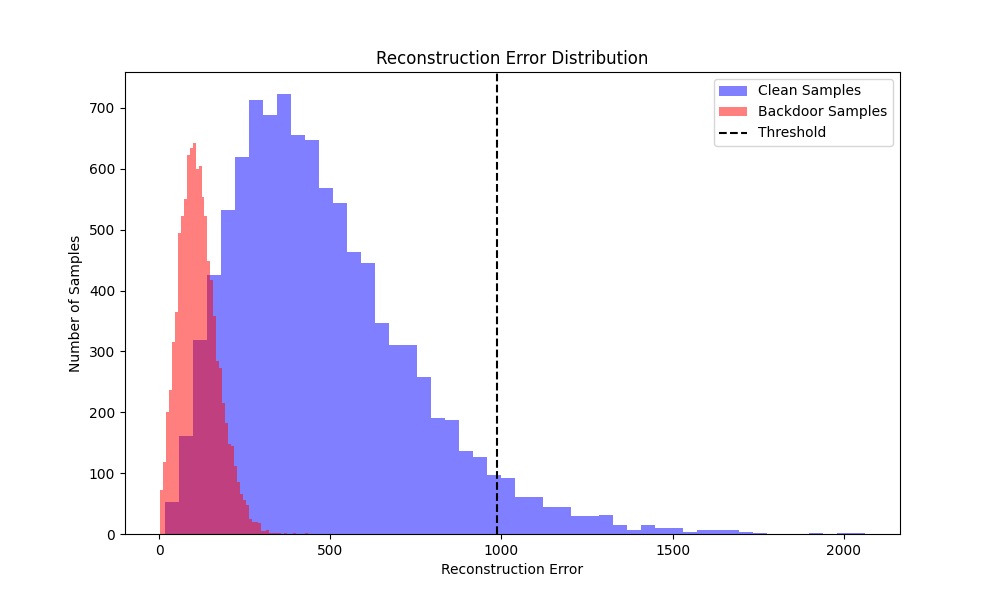
\includegraphics{Figs/error_distribution.pdf}
    }
    \vspace{-0.2cm}
    \caption{Reconstruction error of DeDe~\cite{hou2025dede} on INACTIVE invisible poisoned samples. The threshold is set to the 99.5\textsuperscript{th} percentile of the clean reconstruction error. All INACTIVE poisoned samples lie below this threshold, making them undetectable by DeDe.}
    \label{fig:dede_inactive}
\end{figure}


\begin{figure}[!ht]
\centering
\begin{rqconclusion}{Conclusion for RQs 1-2}
\textit{\texttt{LoREx} achieves robust detection across the tested attack scenarios considered.}
\end{rqconclusion}
\vspace{-0.25cm}
\end{figure}

\begin{table*}[!ht]
\centering
\caption{Downstream classification performance. \textbf{CA}: Clean Accuracy ($\uparrow$), \textbf{ASR}: Attack Success Rate ($\downarrow$). The best results are in bold.}
\begin{tabular}{llcccccccc}
\toprule
\textbf{Target} & \multirow{2}{*}{\textbf{Defense}} & \multicolumn{2}{c}{\textbf{BadEncoder}} & \multicolumn{2}{c}{\textbf{DRUPE}} & \multicolumn{2}{c}{\textbf{INACTIVE}} & \multicolumn{2}{c}{\textbf{BadCLIP}} \\
\cmidrule(lr){3-4} \cmidrule(lr){5-6} \cmidrule(lr){7-8} \cmidrule(lr){9-10}
\textbf{Model} & & CA($\uparrow$) & ASR($\downarrow$) & CA & ASR & CA & ASR & CA & ASR \\
\midrule\midrule
\multirow{4}{*}{SimCLR} 
 & No def. & 86.4 & 99.9 & 85.5 & 96.3 & 86.2 & 99.9 & - & - \\
 & ASSET~\cite{asset} & 86.3 & 55.3 & 85.9 & 53.7 & 86.1 & 99.9 & - & - \\
 & DeDe~\cite{hou2025dede} & 86.5 & 1.3 & 85.9 & 2.1 & 86.2 & 99.9 & - & - \\
 & \texttt{LoREx} & \underline{\textbf{86.4}} & \underline{\textbf{0.0}} & \underline{\textbf{86.4}} & \underline{\textbf{0.0}} & \underline{\textbf{86.3}} & \underline{\textbf{0.0}} & - & - \\
\midrule
\multirow{4}{*}{CLIP} 
 & No def. & \underline{\textbf{82.4}} & 99.8 & \underline{\textbf{83.5}} & 96.3 & \underline{\textbf{83.9}} & 98.7 & \underline{\textbf{82.8}} & 98.3 \\
 & ASSET & 81.3 & 47.1 & 76.9 & 98.7 & 80.8 & 96.9 & 81.1 & 97.4 \\
 & DeDe & 82.4 & 1.1 & 81.9 & 4.1 & 83.2 & 98.7& 81.6 & 30.5 \\
 & \texttt{LoREx} & 82.3 & \underline{\textbf{1.0}} & 82.4 & \underline{\textbf{1.2}} & 82.3 & \underline{\textbf{0.7}} & 82.3 & \underline{\textbf{1.1}} \\
\bottomrule
\end{tabular}%
\label{tab:downstream_performance}
\end{table*}

\paragraph{Downstream Task Performance (RQ3).}
RQ3 examines whether filtering improves downstream robustness without harming model utility. 
We remove the samples flagged by each defense and retrain downstream classifiers on the resulting dataset. 
Table~\ref{tab:downstream_performance} reports CA and ASR after filtering. 
\texttt{LoREx} maintains clean accuracy within 0.2\% of the undefended baseline and reduces ASR to at most 1.2\% across the evaluated attacks. 
For comparison, ASSET lowers clean accuracy due to a higher false positive rate, while DeDe's thresholding does not identify INACTIVE samples.


% The results expose a fundamental trade-off that \texttt{LoREx} successfully resolves. ASSET reduces ASR in some cases, but its high false positive rate damages utility considerably. On DRUPE with CLIP, CA drops from 83.5\% to 76.9\% because ASSET incorrectly discards 28.5\% of the clean samples. Among three defenses, ASSET consistently preserves least CA. DeDe preserves utility by maintaining low false positives, but this conservative approach allows attacks to persist. INACTIVE retains 99.9\% ASR on SimCLR and 98.7\% on CLIP because DeDe cannot detect it at all.

The results highlight how the defenses differ in handling the trade-off between false positives and missed detections. 
\texttt{LoREx} achieves both low ASR and high CA by identifying poisoned samples without discarding many clean ones. 
ASSET reduces ASR in some settings, but its higher false positive rate lowers utility; for example, on DRUPE with CLIP, CA drops from 83.5\% to 76.9\% because it removes 28.5\% of the clean samples. 
Across the three defenses, ASSET shows the largest reduction in CA. 
DeDe maintains utility by keeping false positives low, but this also leaves certain attacks unfiltered. 
For INACTIVE, ASR stays at 99.9\% on SimCLR and 98.7\% on CLIP because DeDe does not detect these samples.


\texttt{LoREx} meets both goals: reducing ASR and preserving clean utility. 
Its spectral separation identifies the trigger-related dimensions, bringing ASR down to at most 1.2\% across the evaluated attacks. 
At the same time, CA remains within 0.2\% of the undefended baseline. 
These results indicate that whitening-based detection can isolate poisoned samples effectively while retaining almost all useful data.


\begin{figure}[H]
\centering
\begin{rqconclusion}{Conclusion for RQ3}
\textit{Filtering based on \texttt{LoREx} detection detects backdoors successfully without sacrificing model utility.}
\end{rqconclusion}
\vspace{-0.25cm}
\end{figure}
\subsection{Defense Resource Requirements (RQ4)}
\label{exp_resource}

\begin{table}[h]
    \centering
    \caption{Resource consumption on CIFAR-10 (ResNet-18). Memory is measured as VRAM for GPU methods and RAM for CPU methods. Latency is per-sample average during inference.}
    \label{tab:resource_benchmarks}
    \resizebox{\columnwidth}{!}{
    \begin{tabular}{lccc}
        \toprule
        \textbf{Metric} & \textbf{ASSET}~\cite{asset} & \textbf{DeDe}~\cite{hou2025dede} & \textbf{\texttt{LoREx}} \\
        \midrule
        \multicolumn{4}{l}{\textit{Phase I: Preparation}} \\
        Running Time & $\approx$ 45 min & $\approx$ 2.5 hr & \textbf{1.8 sec} \\
        Memory & $\sim$ 6 GB GPU & $\sim$ 10 GB GPU & \textbf{$\sim$ 0.2 GB CPU} \\
        \midrule
        \multicolumn{4}{l}{\textit{Phase II: Inference}} \\
        Latency Overhead & N/A (Offline) & +83\% ($\sim$22 ms) & \textbf{$<$0.01 ms} \\
        Storage & N/A & $\sim$ 45 MB & \textbf{1 MB} \\
        \bottomrule
    \end{tabular}
    }
\end{table}

Having shown the detection performance of \texttt{LoREx}, we next examine its computational cost. 
Scalability is an important factor as SSL models continue to increase in size and are used in a wider range of settings~\cite{abad2025soklinedefensebackdoor}. 
Defenses that require sophisticated optimization introduce additional overhead during preparation and limit how easily they can be applied at inference time.


Table~\ref{tab:resource_benchmarks} compares resource usage across two phases: preparation (calibration before deployment) and inference (real-time filtering).

In the preparation phase, the methods differ mainly in computational cost. 
ASSET's bi-level optimization takes about 45 minutes and uses 6~GB of VRAM, while DeDe's decoder training takes roughly 2.5 hours and uses 10~GB of VRAM. 
\texttt{LoREx}, which relies on covariance estimation and eigendecomposition, completes this step in 1.8 seconds using 0.2~GB of RAM.

The inference phase shows a similar contrast. 
ASSET operates only offline and does not provide inference-time protection. 
DeDe requires both encoder and decoder passes, adding 83\% latency per sample. 
\texttt{LoREx} performs detection through a matrix-vector multiplication ($\mathcal{O}(d^2)$), adding less than 0.01~ms, which is negligible compared to the encoder's forward pass.

These differences follow from the underlying design choices. Optimization-based and reconstruction-based defenses depend on iterative training, which scales with model size and data volume. 
In contrast, \texttt{LoREx} uses a fixed linear transformation based on ZCA whitening, requiring only covariance estimation and matrix factorization. 
This allows fast encoder auditing and low-latency filtering at inference time, and its detection threshold can be updated by recomputing clean embedding statistics without retraining or modifying the SSL encoder.


\begin{figure}[H]
\centering
\begin{rqconclusion}{Conclusion for RQ4}
\textit{\texttt{LoREx} executes in seconds at an affordable computational cost.}
\end{rqconclusion}
\vspace{-0.25cm}
\end{figure}

\subsection{Adaptive Attack Robustness (RQ5)}
\label{exp_adaptive}
A thorough security evaluation must include adaptive adversaries with full knowledge of the defense. 
We assume the attacker has access to a shadow dataset for estimating $\bm{\Sigma}_c$, full knowledge of the whitening procedure, and the ability to adjust the attack objective accordingly. 
Under this setting, the attacker identifies the low-variance eigenvectors $\mathbf{U}_{low}$ and attempts to reduce the trigger signal along these directions. 
We evaluate three adaptive strategies.

\textbf{Regularized Training} penalizes trigger energy in monitored subspaces:
$\mathcal{L}_{total} = \mathcal{L}_{target} + \lambda_c \mathcal{L}_{clean} + \lambda_{ev} \| (\mathbf{z}_{poison} - \mathbf{z}_{benign}) \cdot \mathbf{U}_{low} \|_2$ where $\mathcal{L}_{total}$ is the optimization objective function, $\mathcal{L}_{target}$ and $\mathcal{L}_{clean}$ denote the cosine distance between poisoned embeddings and target embeddings, and between poisoned embeddings and clean embeddings, respectively. $\lambda_c$ and $\lambda_{ev}$ are coefficients that control the contributions of the loss function components. $\mathbf{z}_{poison}$ and $\mathbf{z}_{benign}$ are the poisoned and benign embeddings, respectively. $\mathbf{U}_{low}$ is the matrix of eigenvectors corresponding to the low-variance dimensions.

% \mn{the lambdas are not clarified well}

\textbf{High-Variance Targeting} explicitly embeds triggers into high-variance dimensions:
$\mathcal{L}_{total} = \mathcal{L}_{target} + \lambda_c \mathcal{L}_{clean} - \lambda_{hv} \| (\mathbf{z}_{poison} - \mathbf{z}_{benign}) \cdot \mathbf{U}_{high} \|_2$. Here, $\lambda_{hv}$ is the coefficient of the high-variance alignment component in the loss function and $\mathbf{U}_{high}$ is the matrix of eigenvectors corresponding to the high-variance dimensions.

% \mn{this formulation is unclear}

\textbf{Generative Trigger Synthesis} uses a learned U-Net generator $G$ producing sample-specific perturbations: 
$\min_{G, f_\alpha} \mathcal{L}_{target} + \lambda_c \mathcal{L}_{clean} + \lambda_{ev} \mathcal{L}_{evasion} + \lambda_p \|G(\mathbf{x}) - \mathbf{x}\|_2$ where $\mathbf{x}$ is the input image and $\mathcal{L}_{evasion}$ is the loss for the triggered embedding's stealthiness, calculated by aligning the poisoned embedding distribution to match with the clean distribution, following DRUPE~\cite{tao2024distribution}. The final term $\|G(\mathbf{x}) - \mathbf{x}\|_2$ penalizes the added trigger's visibility to avoid detection by visual inspection.

\begin{table}[t]
    \centering
    \caption{Adaptive attack evaluation on CIFAR-10 with SimCLR. Evasion attempts that reduce detection simultaneously collapse attack effectiveness, confirming the stealth-efficacy dilemma.}
    \label{tab:adaptive_attack}
    \resizebox{\columnwidth}{!}{
    \begin{tabular}{lccc}
        \toprule
        \textbf{Attack Strategy} & \textbf{ASR} ($\downarrow$) & \textbf{CA} ($\uparrow$) & \textbf{Detection TPR} ($\uparrow$) \\
        \midrule
        Regularized Training & 11.7\% & 84.2\% & 93.6\% \\
        High-Variance Targeting & 18.9\% & 83.5\% & 91.2\% \\
        Generative (UNet) & 5.8\% & 81.7\% & 88.4\% \\
        \bottomrule
    \end{tabular}
    }
\end{table}

Table~\ref{tab:adaptive_attack} shows a consistent trend across all strategies: lowering detection rates reduces attack effectiveness. 
Regularized Training decreases detection TPR to 93.6\%, but ASR also drops to 11.7\% because the evasion and backdoor objectives place opposing constraints on the trigger. 
To remain effective, the trigger must produce a consistent embedding shift, while evasion requires keeping its energy low in the monitored subspace. 
High-Variance Targeting reaches 91.2\% TPR with 18.9\% ASR; placing the trigger in high-variance directions mixes it with natural variation, reducing its consistency. 
The Generative approach achieves the lowest detection (88.4\% TPR), but ASR falls to 5.8\%, reflecting the same conflict between generating an effective and an inconspicuous trigger.

These observations align with the analysis in Section~\ref{motivation}. 
Backdoors depend on low-rank, consistent signals that avoid dominant semantic dimensions. 
Shifting the trigger into high-variance regions increases overlap with natural variability and weakens its reliability. 
Thus, the attacker faces a structural limitation: the conditions that enable stealth also make the trigger detectable once whitening is applied.


\begin{figure}[H]
\centering
\begin{rqconclusion}{Conclusion for RQ5}
\textit{In our experiments, adaptive attackers with full defense knowledge could not evade \texttt{LoREx} without degrading attack effectiveness.}
\end{rqconclusion}
\vspace{-0.25cm}
\end{figure}

\subsection{Empirical Validation of Whitening Hypothesis (RQ6)}
\label{exp_analysis}
The previous experiments show that \texttt{LoREx} achieves reliable detection, but they do not directly validate the mechanism underlying the method. 
We therefore examine whether whitening produces the geometric effects predicted by our analysis. 
We evaluate three predictions: (i) whitening makes the clean distribution closer to isotropic, 
(ii) trigger signals located in low-variance subspaces become larger relative to semantic components, 
and (iii) this amplification increases the separation between clean and poisoned samples.

We use INACTIVE as the main test case because it is designed to conceal triggers by projecting them into low-variance dimensions, making it a strong setting for examining the whitening hypothesis.

\paragraph{Prediction 1: Whitening induces isotropy.}
Figure~\ref{fig:diagonal_after_whitening} (top row) shows the covariance of trusted clean data before and after whitening. 
The unwhitened covariance contains off-diagonal correlations and unequal variances across dimensions, indicating anisotropy in the embedding space. 
After applying $\mathbf{W} = \bm{\Sigma}^{-1/2}$, the covariance approaches identity ($\mathbf{W}\bm{\Sigma}\mathbf{W}^\top \approx \mathbf{I}$), consistent with decorrelation and variance normalization. 
The mixed dataset (bottom row) shows the same pattern: even with poisoned samples present, the whitened covariance remains close to identity, indicating that the reference-based estimate generalizes to the test data.


\begin{figure}[!ht]
    \centering
    \resizebox{0.99\linewidth}{!}{
    \begin{tabular}{c}
        \includegraphics[width=0.90\linewidth]{Figs/clean_cov.pdf} \\
        \textbf{(a) Trusted clean dataset} \\[0.8em]
        \includegraphics[width=0.90\linewidth]{Figs/mixed_cov.pdf} \\
        \textbf{(b) Mixed validating dataset}
    \end{tabular}
    }
    \vspace{-0.3cm}
    \caption{Covariance matrices before (left) and after (right) whitening for the trusted clean dataset (a) and mixed dataset (b). Whitening transforms the anisotropic covariance structure toward identity. For readability, we only visualize the top 25 dimensions.}
    \label{fig:diagonal_after_whitening}
\end{figure}


\paragraph{Prediction 2: Trigger signals are amplified.}
Figure~\ref{fig:eigenvalue_comparison} shows the eigenvalue distribution in the whitened space. 
Clean samples have relatively uniform eigenvalues, consistent with an approximately isotropic distribution. 
Poisoned samples exhibit increased variance along specific dimensions. 
As described in Proposition~\ref{prop1}, whitening scales each direction by $1/\sqrt{\lambda_i}$, so dimensions with smaller $\lambda_i$ receive larger scaling factors. 
The observed variance increases in poisoned samples match this expected amplification of low-variance components.

\begin{figure}[!ht]
     \centering
     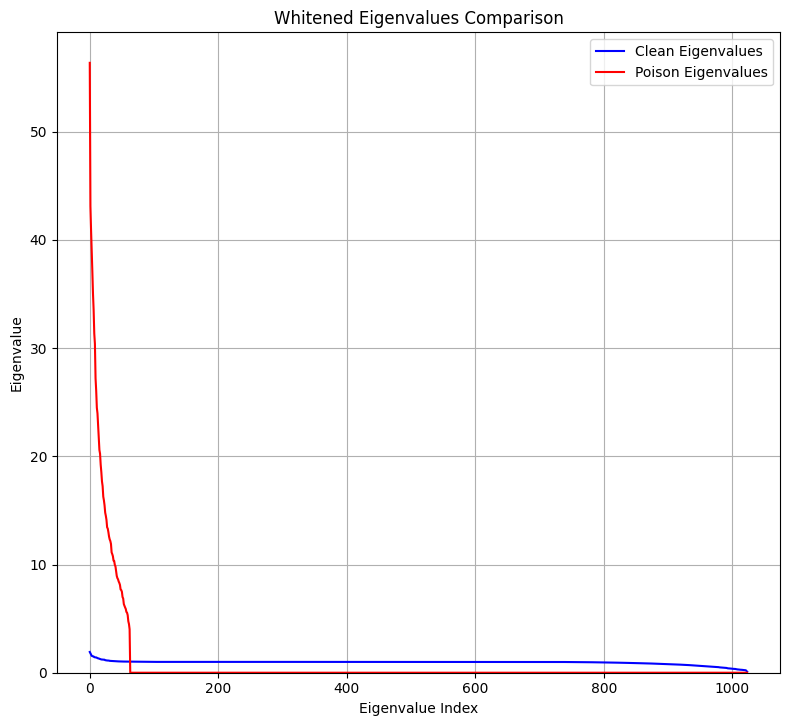
\includegraphics[width=0.99\linewidth]{Figs/eigenvalue_comparison.pdf}
     \vspace{-0.4cm}
     \caption{Eigenvalue distribution in whitened space. Clean samples (blue) show relatively uniform variance across components; poisoned samples (red) show elevated variance along specific directions.}
     \label{fig:eigenvalue_comparison}
\end{figure}

\paragraph{Prediction 3: Amplification produces geometric separation.}
Figure~\ref{fig:3d_pca} visualizes whitened embeddings projected onto their principal components and the backdoor axis $\mathbf{v}_{bd}$ identified by \texttt{LoREx}. 
Clean embeddings remain near the origin, while INACTIVE embeddings shift along the principal directions. 
The pairwise scatter plots in Figure~\ref{fig:pca_matrix} show the same pattern across multiple component pairs and the backdoor axis (“bd\_axis” in the figure). 
These observations indicate that poisoned samples occupy a distinct region in the whitened space.

\begin{figure}[!ht]
    \centering
    \resizebox{0.99\columnwidth}{!}{
        \includegraphics{Figs/3d.pdf}
    }
    % \vspace{-1.6cm}
    \caption{Projection onto top-3 principal components after whitening. INACTIVE samples (red) cluster separately from clean samples (blue) along the backdoor axis (highest variance after whitening).}
    \label{fig:3d_pca}
\end{figure}





These observations align with the proposed mechanism. 
Triggers placed in low-variance subspaces receive larger scaling factors under whitening ($1/\sqrt{\lambda_i}$), which increases their contribution in the transformed space. 
As a result, the trigger becomes a dominant source of variance, leading to the observed geometric separation between clean and poisoned samples.


\begin{figure}[H]
\centering
\begin{rqconclusion}{Conclusion for RQ6}
\textit{The empirical observations are consistent with our theoretical predictions.}
\end{rqconclusion}
\vspace{-0.25cm}
\end{figure}

\begin{figure}[!ht]
    \centering
    \resizebox{0.99\linewidth}{!}{
        \includegraphics{Figs/scatter.pdf}
    }
    \vspace{-.6cm}
    \caption{Pairwise scatter plots of top-3 principal components and the detected backdoor axis (``bd\_axis'') in whitened space. Poisoned samples (red) show consistent displacement from clean samples (blue) along backdoor axis.}
    \label{fig:pca_matrix}
\end{figure}

\subsection{Label-Flipping Experiment}
\label{finding_experiment}
The backdoored model and poisoned samples used in this experiment are adopted from DRUPE~\cite{tao2024distribution}, a backdoor attack that specifically utilizes distributional properties to enhance embedding stealthiness. The experiment is designed as follows: 

\begin{itemize}[leftmargin=0pt]
    \item \textbf{Step 1 - Dataset acquisition:} We construct a training dataset containing clean samples of all available classes and a number of poisoned samples with the trigger applied.
    \item \textbf{Step 2 - Target label randomization:} we reassign the labels of all poisoned samples to a single randomly chosen class that differs from both their original semantic class and the attacker's chosen target class. Clean sample labels remain unchanged.
    \item \textbf{Step 3 - Embedding extraction:} We then feed these images to the backdoored encoder to extract their embeddings. At this point, we have constructed a dataset that resembles a downstream classifier training dataset, except for the addition of poisoned samples, which have their target labels randomized.
    \item \textbf{Step 4 - Classifier training:} We train multiple simple classifiers---Decision Tree~\cite{breiman2017classification}, Support Vector Machine (SVM)~\cite{cortes1995support}, Logistic Regression~\cite{montgomery2021introduction}, and Multilayer Perceptron (MLP)~\cite{rumelhart1986learning}---on the extracted embedding dataset and observe their classification results.
\end{itemize}
\begin{table}[h]
\centering
\caption{Performance of simple downstream models with target labels randomized for poisoned samples.}
\label{tab:finding_experiment}
% Resizes table to exact column width
\resizebox{\columnwidth}{!}{%
\begin{tabular}{lcc}
\toprule
\textbf{Model} & \textbf{Poison Acc.} & \textbf{Clean Acc.} \\
\midrule
Decision Tree~\cite{breiman2017classification}      & 98.87\% & 88.51\% \\
SVM~\cite{cortes1995support}                        & 98.92\% & 89.51\% \\
MLP~\cite{rumelhart1986learning}                    & 99.17\% & 88.13\% \\
Logistic Regression~\cite{montgomery2021introduction} & 98.84\% & 89.24\% \\
\bottomrule
\end{tabular}%
}
\end{table}

Table~\ref{tab:finding_experiment} shows that all downstream classifiers reach ${\sim}99\%$ accuracy on poisoned samples, even though these samples are assigned labels being unrelated to the attacker's target class or the original image content. 
This performance is about 10 percentage points higher than the accuracy on clean samples (${\sim}88$-$89\%$). Logistic Regression, a linear classifier, achieves 98.84\% poison accuracy, indicating that the poisoned embeddings are approximately linearly separable from clean embeddings. Furthermore, all four classifiers achieve similar poison accuracy, suggesting that the separation reflects a property of the embedding geometry, not a specific behavior of a particular classifier.
Because the target labels are randomized, the high accuracy on poisoned samples cannot be explained by memorization of specific image-trigger-label combinations. 
Instead, the results suggest that the backdoored encoder maps trigger-containing inputs to a distinct region in embedding space, independent of semantics. 
The observed linear separability is consistent with our theoretical analysis, where the trigger induces a consistent displacement along a small number of embedding dimensions.


\section{Related Work}
\label{Section7}

\par \textbf{Spectral defenses in supervised learning.}
Spectral Signatures~\cite{tran2018spectral} first observed that poisoned samples leave detectable artifacts in representation covariance. The method computes the top singular vector within each class and removes outliers along this direction. SCAn~\cite{tang2021demon} extends this idea using expectation-maximization (EM)-based decomposition to detect mixture distributions within classes, improving robustness to blended attacks. Both methods share a critical requirement: class labels are essential for partitioning data before spectral analysis. In SSL, labels are unavailable and encoders produce task-agnostic embeddings, rendering within-class analysis inapplicable. \texttt{LoREx} instead operates on the global covariance of unlabeled embeddings, exploiting the insight that SSL triggers hide in low-variance subspaces of the clean distribution rather than within a target class.

\par \textbf{Activation and behavioral methods.}
Activation Clustering (AC)~\cite{chen2018detecting} identifies backdoors by detecting bimodal structure in final-layer activations of a trained classifier. STRIP~\cite{gao2019strip} perturbs inputs at inference time and flags samples with low prediction entropy as triggered. Both approaches fundamentally rely on classifier outputs: AC requires class-specific activations, and STRIP requires discrete predictions to compute entropy. SSL encoders produce continuous embeddings without class structure, eliminating the signals these methods exploit. Applying these methods to SSL would require first training a downstream classifier, shifting detection to post-deployment rather than encoder auditing.

\par \textbf{Positioning of \texttt{LoREx}.}
Prior spectral and statistical defenses were designed for supervised learning, where labels enable within-class analysis and classifiers produce discrete predictions. \texttt{LoREx} addresses SSL backdoor detection by shifting from within-class spectral analysis to global whitening, retaining the core insight that backdoors leave low-rank signatures while eliminating the label dependency.

\section{Discussion}
\label{Section8}

\par \textbf{Impact of the Study.} This work shows that spectral patterns in SSL embeddings can reliably reveal backdoor triggers. Using this insight, \texttt{LoREx} provides a lightweight method for auditing SSL encoders under practical resource limits. Our analysis also identifies a geometric trade-off between trigger stealth and effectiveness. This helps characterize how SSL backdoors operate. These findings offer a useful basis for developing more efficient and robust defenses. 

\par \textbf{Limitations.}
\texttt{LoREx} requires access to a small set of trusted clean samples to estimate the clean covariance matrix. Although our experiments show that using only 1\% of the training data is sufficient, scenarios with no clean data would require alternative strategies, such as estimating the covariance from the mixed set with a robust outlier-filtering step. The method also relies on the standard assumption used in prior backdoor analyses that trigger features occupy low-variance directions relative to the clean distribution. This assumption reflects how existing backdoor attacks are constructed in practice. Developing defenses that do not rely on this assumption remains an open direction.


\par \textbf{Future Work.} While \texttt{LoREx} shows robustness against the adaptive backdoor attacks evaluated in Section~\ref{exp_adaptive}, attackers may design new strategies that specifically target its whitening-based detection. We outline two interesting directions of future work: (1) constructing source-specific backdoors by aligning the trigger with features of a chosen class, and (2) spreading the trigger signal more uniformly across embedding dimensions to reduce its concentration in low-variance directions. Approach (1) tends to weaken during downstream fine-tuning, as noted in prior work~\cite{hou2025dede}, while approach (2) may overly dilute the trigger signal and reduce its impact. Other research directions include: (i) extending \texttt{LoREx} to multi-modal SSL encoders (e.g., audio and text), and (ii) deriving bounds on the minimum trigger magnitude that remains detectable under different data and model conditions.

\section{Conclusion}
\label{Section9}
We introduce \texttt{LoREx}, a lightweight and attack-agnostic method for detecting backdoor attacks in SSL encoders. The method relies on a simple observation: current backdoor attacks place their trigger features in low-variance directions of the clean embedding space. Whitening amplifies these low-variance components and suppresses high-variance semantic directions, which exposes the trigger signal. \texttt{LoREx} achieves high detection accuracy (AUC $>0.99$) on four state-of-the-art attacks with two encoders: SimCLR and CLIP. \texttt{LoREx} also lowers attack success rates from above 95\% to below 2\%. The method is computationally efficient as it is training-free.

 
\section*{Ethical Considerations and Compliance with the Open Science Policy}

\section*{Ethical Considerations}
\par This study does not use any sensitive data regarding privacy and security. We use open-source datasets to conduct our experiments. This research was conducted with a commitment to upholding the highest ethical standards. The methodologies employed were carefully designed to ensure that the research respects the privacy and rights of individuals, avoids bias, and minimizes potential harm. Data used in the study was sourced and managed responsibly, adhering to ethical guidelines that prioritize confidentiality and the ethical use of information. The research aims to contribute positively to defending against backdoor attacks towards Safe, Secure, and Trustworthy AI. 

\section*{Open Science}
\par In accordance with the open science policy, this research fully embraces transparency and reproducibility. All source code developed during the project has been anonymously shared, ensuring accessibility for validation and further research. We have made every effort to provide detailed documentation and descriptions of our work to facilitate its implementation and reproducibility by others in both research and practice communities. By adhering to these open science principles, we aim to contribute meaningfully to the advancement of knowledge while maintaining the integrity and openness that are essential to scientific progress. The source code can be found at the following anonymized link:~\url{https://anonymous.4open.science/r/LoREx}.


\bibliographystyle{unsrt}
\bibliography{references.bib}

\appendix

% \mn{This is too verbose; a math proof has to be more direct to the point and more mathematically based.}

\section{Proof of Whitening Amplification}
\label{appendix:proof}

We prove Proposition~\ref{prop1}. Assume zero-mean embeddings (achieved by centering).

\par \textbf{Setup.} Let $\mathbf{z}_b \in \mathbb{R}^d$ be a benign embedding with covariance $\bm{\Sigma} = \mathbb{E}[\mathbf{z}_b \mathbf{z}_b^\top]$. A poisoned embedding decomposes as $\mathbf{z}_p \approx \mathbf{z}_c + \mathbf{z}_t$, where $\mathbf{z}_c$ is the clean semantic component (distributed as $\mathbf{z}_b$) and $\mathbf{z}_t$ is the trigger artifact. 

\par \textbf{Assumptions.}
\begin{enumerate}[label=(A\arabic*), leftmargin=*, topsep=2pt, itemsep=1pt]
    \item \textit{Uncorrelated components:} $\mathbb{E}[\mathbf{z}_c \mathbf{z}_t^\top] = \mathbf{0}$. Stealth requires triggers orthogonal to semantic variation; correlated components would shift embeddings along semantic directions, producing detectable distributional changes~\cite{tao2024distribution,zhang2025invisible}.
    \item \textit{Low-variance concentration:} $\mathbf{z}_t$ concentrates energy in directions with small eigenvalues of $\bm{\Sigma}$. High-variance directions capture dominant semantic features; triggers there would disrupt clean semantics and be detectable by simple statistics~\cite{tran2018spectral}.
\end{enumerate}

\par \textbf{Whitening transformation.} Define $\mathbf{W} = \bm{\Sigma}^{-1/2} = \mathbf{U}\bm{\Lambda}^{-1/2}\mathbf{U}^\top$ where $\bm{\Sigma} = \mathbf{U}\bm{\Lambda} \mathbf{U}^\top$ is the eigendecomposition with $\bm{\Lambda} = \mathrm{diag}(\lambda_1, \ldots, \lambda_d)$. This transformation satisfies $\mathbf{W}\bm{\Sigma} \mathbf{W}^\top = \mathbf{I}$, normalizing each principal direction to unit variance.

\par \textbf{Benign embeddings.} The whitened covariance is identity, so the expected squared norm equals the sum of $d$ unit variances:
\begin{equation}
\mathbb{E}[\|\mathbf{W}\mathbf{z}_b\|_2^2] = \mathrm{tr}(\mathbf{W}\bm{\Sigma} \mathbf{W}^\top) = \mathrm{tr}(\mathbf{I}) = d.
\end{equation}

\par \textbf{Poisoned embeddings.} Since $\mathbf{W}\mathbf{z}_p = \mathbf{W}\mathbf{z}_c + \mathbf{W}\mathbf{z}_t$:
\begin{equation}
\|\mathbf{W}\mathbf{z}_p\|_2^2 = \|\mathbf{W}\mathbf{z}_c\|_2^2 + \|\mathbf{W}\mathbf{z}_t\|_2^2 + 2(\mathbf{W}\mathbf{z}_c)^\top(\mathbf{W}\mathbf{z}_t).
\end{equation}
Taking expectations and applying (A1):
\begin{equation}
\mathbb{E}[(\mathbf{W}\mathbf{z}_c)^\top(\mathbf{W}\mathbf{z}_t)] = \mathbb{E}[\mathbf{z}_c^\top \bm{\Sigma}^{-1} \mathbf{z}_t] = \mathrm{tr}(\bm{\Sigma}^{-1}\mathbb{E}[\mathbf{z}_c \mathbf{z}_t^\top]) = 0.
\end{equation}
Since $\mathbf{z}_c$ follows the benign distribution, $\mathbb{E}[\|\mathbf{W}\mathbf{z}_c\|_2^2] = d$. Thus:
\begin{equation}
\mathbb{E}[\|\mathbf{W}\mathbf{z}_p\|_2^2] = d + \mathbb{E}[\|\mathbf{W}\mathbf{z}_t\|_2^2].
\end{equation}

% \mn{Please consistently format the symbols denoting vectors and matrices in bold-face.}

The whitened trigger norm expands as:
\begin{equation}
\|\mathbf{W}\mathbf{z}_t\|_2^2 = \mathbf{z}_t^\top \bm{\Sigma}^{-1} \mathbf{z}_t = \sum_{i=1}^{d} \frac{(\mathbf{u}_i^\top \mathbf{z}_t)^2}{\lambda_i}.
\end{equation}
The term $(\mathbf{u}_i^\top \mathbf{z}_t)^2$ is the squared projection of the trigger onto eigenvector $\mathbf{u}_i$, and $\lambda_i$ is the benign variance in that direction. For low-variance directions where $\lambda_i$ is small, the factor $1/\lambda_i$ becomes large. By (A2), trigger energy concentrates in the $k$ smallest eigenvalue directions. Let $\tau^2 = \mathbb{E}[\|\mathbf{z}_t\|_2^2]$ and $\lambda_{\max}^{(k)} = \max_{i > d-k} \lambda_i$. Then:
\begin{equation}
\mathbb{E}[\|\mathbf{W}\mathbf{z}_t\|_2^2] \ge \sum_{i=d-k+1}^{d} \frac{\mathbb{E}[(\mathbf{u}_i^\top \mathbf{z}_t)^2]}{\lambda_i} \geq \frac{\tau^2}{\lambda_{\max}^{(k)}}.
\end{equation}
When $\lambda_{\max}^{(k)} \ll 1$, a small raw trigger magnitude $\tau$ produces $\mathbb{E}[\|\mathbf{W}\mathbf{z}_t\|^2] \gg \tau^2$.

\par \textbf{Separation.} When $\tau^2/\lambda_{\max}^{(k)} \gg d$:
\begin{equation}
\mathbb{E}[\|\mathbf{W}\mathbf{z}_p\|_2^2] = d + \mathbb{E}[\|\mathbf{W}\mathbf{z}_t\|_2^2] \gg d = \mathbb{E}[\|\mathbf{W}\mathbf{z}_b\|_2^2]. \quad \square
\end{equation}

\par \textbf{Remark (Regularization).} When $\bm{\Sigma}$ is ill-conditioned, we use $\mathbf{W} = \mathbf{U}(\bm{\Lambda} + \epsilon \mathbf{I})^{-1/2}\mathbf{U}^\top$ with $\epsilon > 0$. This bounds amplification at $1/\sqrt{\epsilon}$ while preserving the qualitative behavior. Importantly, regularization ensures $\mathbf{W}$ is not orthogonal to directions where triggers reside: any direction with $\lambda_i < \epsilon$ receives amplification $(\lambda_i + \epsilon)^{-1/2} \geq \epsilon^{-1/2}$, guaranteeing trigger signals are amplified rather than suppressed. We use $\epsilon = 10^{-8}$ in experiments.

% \section{Proof of Whitening Amplification}
% \label{appendix:proof}
 

% We provide the complete proof of Proposition~\ref{prop1}. 
% \par \textbf{Presumption}
% The proof is built on a presumption that a poisoned embedding can be decomposed as: $E_{poisoned}\approx E_{clean}+E_{trigger}$. This presumption can be reasonably derived from the constraint that the backdoored encoder must behave normally without the trigger. To satisfy this, $E_{clean}$ and $E_{trigger}$ should be statistically independent (or weakly correlated), as the trigger is designed to not disrupt clean semantics significantly. Since the clean component $E_{clean}$ has already spanned along high-rank dimensions with higher variation in order to mimic the clean features, the trigger component $E_{trigger}$ should sneak in lower-rank dimensions with lower variation for stealthy signal. From there, we can approximate the covariance of poisoned embeddings by the additive relation of clean component and trigger component's covariance: 
% \begin{equation}
% \Sigma_{poisoned}\approx\Sigma_{clean}+\Sigma_{trigger}
% \end{equation}
% And thus the approximation of poisoned embedding as:
% \begin{equation}
% E_{poisoned}\approx E_{clean}+E_{trigger}
% \end{equation}
% On the other hand, the benign embedding does not contain the trigger component and thus can be approximate as:
% $E_{benign}\approx E_{clean}$

% \par \textbf{Setup.}
% Let the benign embedding be a random variable $x_b \in \mathbb{R}^d$ with mean $\mu$ and covariance matrix $\Sigma = \mathbb{E}[(x_b-\mu)(x_b-\mu)^T]$. For simplicity, we assume centered data ($\mu=0$). We seek a transformation $y=Wx_b$ such that the covariance of the transformed benign data is the identity matrix $I$.

% \par \textbf{Derivation of the Whitening Matrix.}
% The covariance of the transformed data is:
% \begin{align}
% \text{Cov}(y) &= \mathbb{E}[yy^T] = \mathbb{E}[Wx_bx_b^TW^T] \nonumber \\
% &= W \mathbb{E}[x_bx_b^T] W^T = W\Sigma W^T
% \end{align}

% To satisfy $\text{Cov}(y)=I$, we require $W\Sigma W^T = I$, which is satisfied by $W = \Sigma^{-1/2}$. We construct this via eigendecomposition:
% \begin{equation}
% \Sigma = U\Lambda U^T
% \end{equation}
% where $U$ is the orthogonal matrix of eigenvectors $u_i$ and $\Lambda = \text{diag}(\lambda_1, \ldots, \lambda_d)$ contains the eigenvalues representing variance along each principal component. The whitening matrix is then:
% \begin{equation}
% W = U \Lambda^{-1/2} U^T
% \end{equation}
% \par \textbf{Effect on Poisoned Embeddings.}
% Based on our additive decomposition, a poisoned embedding can be written as:
% \begin{equation}
% x_{p} \approx x_{c} + x_{t}
% \end{equation}
% where $x_{c}$ is the clean semantic component and $x_{t}$ is the trigger artifact. Applying the whitening transformation:
% \begin{equation}
% Wx_{p} \approx W(x_{c} + x_{t}) = Wx_{c} + Wx_{t}
% \end{equation}



% \mn{In Eq.~(11), the second equality is unclear why it should hold: 
% $\Lambda^{-1/2}U^{T} \ne U\Lambda^{-1/2}U^{T}$. Premultiplying by $U$ changes the matrix. This can not be correct unless U is the identity matrix.}
% -> \nhat{The previous equality was a mistake, I forgot to delete the old one ($A^{-1/2}U^T$)}


% Since $x_{c}$ follows the benign distribution, $Wx_{c}$ has covariance $I$ (isotropic with unit variance). The critical term is $Wx_{t}$.

% The squared $L_2$ norm of the whitened trigger is:
% \begin{equation}
% \|Wx_{t}\|^2 = x_{t}^T W^T W x_{t} = x_{t}^T \Sigma^{-1} x_{t}
% \end{equation}

% Substituting the eigendecomposition $\Sigma^{-1} = U \Lambda^{-1} U^T$:
% \begin{equation}
% \|Wx_{t}\|^2 = x_{t}^T U \Lambda^{-1} U^T x_{t} = \sum_{i=1}^{d} \frac{(u_i^T x_{t})^2}{\lambda_i}
% \end{equation}

% The term $(u_i^T x_{t})^2$ represents the squared projection of the trigger onto the $i$-th eigenvector of the clean space, and $\lambda_i$ is the clean variance in that direction.

% \par \textbf{The Stealth-Amplification Trade-off.}
% For a stealthy attack, the trigger $x_{t}$ must avoid disrupting primary semantic features, which correspond to eigenvectors with large eigenvalues. Therefore, the trigger signal resides predominantly in subspaces with small $\lambda_i$. 

% For these low-variance directions, $\lambda_i \rightarrow 0$, causing $1/\lambda_i$ to become very large. Even if the raw trigger magnitude $\|x_{t}\|$ is small (for stealthiness), the whitened magnitude $\|Wx_{t}\|$ is significantly amplified.

% \par \textbf{Conclusion.}
% Combining the above, the norm of the whitened poisoned embedding is:
% \begin{equation}
% \|Wx_p\|^2 = \|Wx_{c} + Wx_{t}\|^2 \approx \|Wx_{c}\|^2 + \|Wx_{t}\|^2 + 2(Wx_c)^T(Wx_t)
% \end{equation}

% Under the independence assumption, the cross-term has zero expectation. Since $\mathbb{E}[\|Wx_{c}\|^2] = d$ (sum of $d$ unit variances) and $\|Wx_{t}\|^2 \gg d$ due to the amplification, we conclude:
% \begin{equation}
% \|Wx_p\| \gg \|Wx_b\|
% \end{equation}

% \par \mn{$\mathbb{E}[\|Wx_{c}\|^2] = d$ (sum of $d$ unit variances) and $\|Wx_{t}\|^2 \gg d$ why? also if the $\mathbb{E}[\|Wx_{c}\|^2] = d$ is true, does this mean that we must know the clean accuracy?} 
% -> \nhat{$\|Wx_{t}\|^2 \gg d$ is explained in the Stealth-Amplification paragraph.}

% \nhat{I dont get it why $\mathbb{E}[\|Wx_{c}\|^2] = d$ relate to clean accuracy}

% \mn{Does not thins defaul to the trivial case that $W x_t$ should be big?. How do we guarantee that the designed $W$ is for example, not orthogonal to $x_t$?}
% -> \nhat{$Wx_t$ is big because $x_t$ lives in the low-rank dimensions (small $\lambda$), so when we whiten these dimension, the factor $1/\lambda$ is big and amplify $x_t$. This only happen to poisoned mixture because for clean mixture, $1/lambda$ match the clean precomputed distribution and get whitened(Both points are mentioned in the proof)}
% \>\nhat{We avoid $W$ orthogonal to $x_t$ by adding small regularizer $W=U(\Lambda + \epsilon I)^{-1/2}U^T$ in the defense design}

% This proves that whitening disproportionately amplifies trigger artifacts, enabling detection via simple norm thresholding. \hfill $\square$

\end{document}

 1. Figure captions and legend: (Done)
 2. All floats (figures, tables) are references in the text: (Done)
 3. All floats are placed suitably: (Done)
 4. All symbols are introduced (Done)
 5. Adding images (Done)
 6. Did we expand all abbreviations once at their first mention in the body (forget about the Abstract)

The notes

0. Rewrite the Abstract -> Done

1. Attack agnoistic: verify it is the case and claim it. (Stress it in the Abstract and the contribution statement) (Nhat and Mahmoud) -> Done

2. We need a solid argument as to why instant-based detection is required (versus model-based). Add this to prior approaches and limitations. Look into the literature -  Nhat and Mahmoud -> Done

3. Adding a qualitative table that lists the main pros and cons of SoTA, you add ticks and checkmarks. -> Partially 

4. More exp on robustness and generalization-- Nhat -> done

5. Review the math carefully - Mahmoud Done

6. Fixing the write-up - Mahmoud and Nhat -> Done

7. Adding arguments and discussions of the implications of the results in Section 6 -> Done

8. Instead of "ours" say LoREx consistently -> Done

9. Fix the fonts in the figures (use bold-face and laerger fonts) -> Done

10. Fix the appendix. Done

11. Section 5 needs surgery  (Mahmoud) Done

12. Shortening Section 4 (the motivation), and thinking whether to keep it as a single section to absorb it as subsection 5.1 (Nhat) -> Done

13. Double check these commonLY FOIRGOTTEN THINGS
a. All abbreviations are expanded only once
b. All symbols are clarified
c. All floats (figures and tables) are properly cited in text
d. All floats are correctly placed near their relevant text
e. Spell, punctuation, and grammatical checks 
f. Printing and proof-reading the manuscript thoroughly
g. checking that all references are correct and most recent (peer reviewed)